% =====================================================================
%  Master thesis -- Volatility Forecasting with Large Language Models
%  Formatting follows the guideline of Jun.-Prof. Dr. Melina Ludolph:
%  A4, 2.5 cm margins, 12 pt, 1.5 line spacing, decimal sections, APA.
% =====================================================================
\documentclass[12pt,a4paper]{article}

% ---------- Layout ----------
\usepackage[a4paper,margin=2.5cm]{geometry}
\usepackage{setspace}
\onehalfspacing
\usepackage[T1]{fontenc}
\usepackage[utf8]{inputenc}
\usepackage{lmodern}
\usepackage[english]{babel}
\usepackage{csquotes}

% ---------- Tables, figures, maths ----------
\usepackage{booktabs}
\usepackage{longtable}
\usepackage{graphicx}
\usepackage{float}
\usepackage{amsmath,amssymb}
\usepackage{caption}
\captionsetup{font=small,labelfont=bf,skip=6pt}
\usepackage{adjustbox}
% Short captions for the List of Tables
\newcommand{\shortcap}[1]{\csname shortcap@#1\endcsname}
\expandafter\def\csname shortcap@tab:descriptive\endcsname{Descriptive statistics of daily returns}
\expandafter\def\csname shortcap@tab:news\endcsname{Summary of the news data}
\expandafter\def\csname shortcap@tab:baseline\endcsname{Out-of-sample accuracy of the baseline models}
\expandafter\def\csname shortcap@tab:news-gjr\endcsname{Out-of-sample accuracy of news-augmented forecasts (GJR-GARCH-t)}
\expandafter\def\csname shortcap@tab:coefficients\endcsname{In-sample estimates of the news adjustment}
\expandafter\def\csname shortcap@tab:app-EWMA-qml\endcsname{News-augmented forecasts, EWMA baseline (QML)}
\expandafter\def\csname shortcap@tab:app-EWMA-ols\endcsname{News-augmented forecasts, EWMA baseline (OLS)}
\expandafter\def\csname shortcap@tab:app-GARCH-N-qml\endcsname{News-augmented forecasts, GARCH-N baseline (QML)}
\expandafter\def\csname shortcap@tab:app-GARCH-N-ols\endcsname{News-augmented forecasts, GARCH-N baseline (OLS)}
\expandafter\def\csname shortcap@tab:app-GARCH-t-qml\endcsname{News-augmented forecasts, GARCH-t baseline (QML)}
\expandafter\def\csname shortcap@tab:app-GARCH-t-ols\endcsname{News-augmented forecasts, GARCH-t baseline (OLS)}
\expandafter\def\csname shortcap@tab:app-GJR-t-qml\endcsname{News-augmented forecasts, GJR-t baseline (QML)}
\expandafter\def\csname shortcap@tab:app-GJR-t-ols\endcsname{News-augmented forecasts, GJR-t baseline (OLS)}
% \thesistable{file}{caption}{label}: table generated in Python, shrunk only if wider than the text
\newcommand{\thesistable}[3]{%
  \begin{table}[htbp]\centering\small
    \caption[\shortcap{#3}]{#2}\label{#3}
    \begin{adjustbox}{max width=\textwidth}\input{#1}\end{adjustbox}
  \end{table}}

% ---------- References (APA style) ----------
\usepackage[style=apa,backend=biber]{biblatex}
\addbibresource{references.bib}

% ---------- Links ----------
\usepackage[hidelinks]{hyperref}
\usepackage{fancyhdr}
\setlength{\headheight}{15pt}

% =====================================================================
\begin{document}

% ---------------------------------------------------------------------
%  Title page (content required by the guideline, Section 3.4)
% ---------------------------------------------------------------------
\begin{titlepage}
  \centering
  \IfFileExists{ovgu_logo.png}{
\includegraphics[width=0.85\textwidth]{ovgu_logo.png}\par}{}
  \vspace{1.2cm}
  {\LARGE\bfseries Otto von Guericke University Magdeburg\par}
  \vspace{0.3cm}
  {\Large\bfseries Faculty of Economics and Management\par}
  \vspace{1.8cm}
  {\LARGE\bfseries Volatility Forecasting with Large Language Models\par}
  \vspace{1.8cm}
  {\large Master thesis submitted in partial fulfillment of the requirements\\
  for the degree of Master of Science\par}
  \vspace{1.8cm}
  {\large Presented by: Md Tanjib Mahmud\\
  Study Program: International Management, Marketing, Entrepreneurship (IMME)\par}
  \vspace{1.5cm}
  {\large Supervisor: Jun.-Prof.\ Dr.\ Melina Ludolph\par}
\end{titlepage}

% ---------------------------------------------------------------------
%  Front matter
% ---------------------------------------------------------------------
\pagestyle{fancy}\fancyhf{}\fancyhead[C]{\small Volatility Forecasting with Large Language Models}\fancyfoot[C]{\thepage}\renewcommand{\headrulewidth}{0.4pt}
\pagenumbering{roman}
\tableofcontents
\newpage
\listoftables
\newpage
\listoffigures
\newpage
\section*{List of Abbreviations}
\addcontentsline{toc}{section}{List of Abbreviations}
\begin{tabular}{@{}p{3.2cm}p{11cm}@{}}
ARCH & Autoregressive conditional heteroskedasticity \\
BERT & Bidirectional Encoder Representations from Transformers \\
DM & Diebold--Mariano (test of equal predictive accuracy) \\
EWMA & Exponentially weighted moving average \\
FNSPID & Financial News and Stock Price Integration Dataset \\
GARCH & Generalised autoregressive conditional heteroskedasticity \\
GJR-GARCH & Asymmetric GARCH model of Glosten, Jagannathan and Runkle \\
LLM & Large language model \\
MSE & Mean squared error \\
NLP & Natural language processing \\
OLS & Ordinary least squares \\
QLIKE & Quasi-likelihood loss function \\
QML & Quasi-maximum likelihood \\
S\&P 500 & Standard \& Poor's 500 stock market index \\
\end{tabular}

\section*{List of Symbols}
\addcontentsline{toc}{section}{List of Symbols}
\begin{tabular}{@{}p{3.2cm}p{11cm}@{}}
$P_t$ & Adjusted closing price on day $t$ \\
$r_t$ & Daily log return in percent \\
$r_t^2$ & Squared return, used as the proxy for the daily variance \\
$\hat\sigma^2_{t}$ & One-day-ahead variance forecast \\
$\hat\sigma^2_{\text{base}}$ & Variance forecast of a baseline model \\
$\hat\sigma^2_{\text{news}}$ & Variance forecast of the news-augmented model \\
$\omega,\ \alpha,\ \beta,\ \gamma$ & Parameters of the GARCH-type models \\
$\lambda$ & Decay factor of the EWMA model (0.94) \\
$n_{i,t}$ & Number of relevant headlines for stock $i$ used on day $t$ \\
$\text{neg}_{i,t}$ & Share of negative relevant headlines \\
$\text{sent}_{i,t}$ & Mean sentiment score of the relevant headlines \\
$c,\ b_1,\ b_2,\ b_3$ & Coefficients of the news adjustment \\
\end{tabular}
\clearpage
\pagenumbering{arabic}

% =====================================================================
\section{Introduction}\label{sec:introduction}
% =====================================================================

\subsection{Motivation}\label{sec:motivation}
Forecasting financial volatility is a core task of financial economics. Volatility forecasts are needed to price options, to set risk limits and capital buffers, and to decide how much of a portfolio should be invested in risky assets. A portfolio manager who hedges an equity position with options needs a view on future volatility to judge whether the option prices are fair. A bank that reports Value-at-Risk needs an estimate of the conditional variance of its trading book. A pension fund that allocates its assets across asset classes weighs expected returns against expected risk. In all three cases, a better volatility forecast leads directly to a better decision.

For decades, the Generalised Autoregressive Conditional Heteroscedasticity (GARCH) family introduced by \textcite{engle1982} and \textcite{bollerslev1986}, together with the Exponentially Weighted Moving Average (EWMA) of the RiskMetrics framework \parencite{riskmetrics1996}, has been the standard toolkit. These models capture the stylised facts of financial returns well, above all volatility clustering: large price changes tend to be followed by further large changes \parencite{mandelbrot1963,cont2001}. The GARCH(1,1) model has become the workhorse of academic research and industry practice because it is simple, robust and hard to beat out of sample \parencite{hansen2005}.

These models, however, use nothing but past prices. They cannot see why prices move. Earnings announcements, regulatory decisions, product failures or analyst downgrades are all reported in the news before, or at the same time as, they show up in returns, yet a price-based model can only react once the shock has appeared in the data. This limitation matters most in turbulent periods, which are exactly the periods in which accurate volatility forecasts are most valuable. The COVID-19 crash of spring 2020 illustrates the point: it was triggered by a public health emergency rather than by a financial market mechanism, and the volatility of most large US stocks rose far beyond what their past returns implied.

At the same time, methods for turning text into numbers have improved considerably. Dictionary-based approaches \parencite{tetlock2007,loughran2011} showed that the tone of news carries information about markets. Transformer-based language models such as BERT \parencite{devlin2019} and its financial variant FinBERT \parencite{araci2019} read text in context and classify it far more accurately than word lists. Large language models have since been shown to extract return-relevant information from news headlines \parencite{lopezlira2023}. This raises the question of whether language-model features can also improve volatility forecasts, a quantity that is driven by the arrival of information rather than by its direction.

\subsection{Research Question and Hypotheses}\label{sec:rq}
This thesis addresses the following research question:

\begin{quote}
\emph{Do news features extracted with a financial language model improve one-day-ahead volatility forecasts of large US stocks beyond GARCH-type and EWMA benchmarks?}
\end{quote}

The question is deliberately narrow. The language model is used as a measurement tool that converts headlines into daily numerical features, and these features are added to established volatility models. The thesis does not ask whether a language model can forecast volatility on its own. To answer the question, three hypotheses are tested.

\textbf{H1 (strong benchmark).} Price-based models are a strong benchmark, and among them the asymmetric GJR-GARCH model with Student-t errors is the most accurate. This follows the evidence of \textcite{hansen2005}, who find that GARCH(1,1) is rarely beaten and that only models with a leverage effect do better for equity returns.

\textbf{H2 (news and variance).} Company-specific news is associated with higher conditional variance beyond what past returns imply. Days after which many relevant headlines appear should show larger squared returns relative to the GARCH forecast. This is consistent with the idea that news arrival attracts investor attention and trading \parencite{barber2008} and with the finding that unusual news predicts market stress \parencite{glasserman2019}.

\textbf{H3 (forecast gains).} Adding FinBERT-based news features improves out-of-sample one-day-ahead forecasts relative to a benchmark that has been recalibrated in the same way. Because GARCH-type models are strong and news is only observed at daily frequency, the gains are expected to be small.

\subsection{Scientific Approach}\label{sec:approach}
The analysis uses daily data for large US stocks. The main sample covers 47 stocks from January 2017 to May 2020, with the out-of-sample evaluation running from January 2018 to May 2020; the period includes the COVID-19 crash. A second sample of 44 stocks for 2022 and 2023, evaluated in 2023, serves as a robustness check in a calmer and more recent period. Headlines come from the FNSPID dataset \parencite{dong2024}. Each headline is scored with FinBERT, filtered for relevance to the stock it is tagged to, and aggregated to three daily features per stock: the number of relevant headlines, the share of negative headlines and the average sentiment score.

Four baseline models produce one-day-ahead variance forecasts: GARCH(1,1) with normal errors, GARCH(1,1) with Student-t errors, GJR-GARCH(1,1) with Student-t errors and EWMA with $\lambda = 0.94$. All are re-estimated every month on an expanding window. The news-augmented forecast multiplies the baseline forecast by an exponential function of the news features. The coefficients are estimated by quasi-maximum likelihood on all data available before the forecast month and are pooled across stocks. Forecasts are compared using the QLIKE and squared-error loss functions and Diebold--Mariano tests. As the fair comparison, the news models are tested against a recalibrated baseline that is fitted in the same way but uses no news features.

\subsection{Main Results}\label{sec:main-results}
The baseline results support H1: GJR-GARCH with Student-t errors is the most accurate model in the main sample and EWMA the least accurate, while the four models are very close in the calmer 2023 sample. The in-sample results support H2: news intensity is strongly and positively related to variance. In the main sample, a single relevant headline raises the expected variance of the next trading day by about 35\%, and the robustness sample shows an effect of the same sign with a smaller size (about 20\%).

The out-of-sample results support H3 only in a limited sense. For the best baseline, news-augmented forecasts achieve lower QLIKE than the recalibrated baseline, and the difference is statistically significant at the 5\% level in both samples; for the weaker EWMA baseline the gains are larger, for the plain GARCH models they are smaller. Against the untouched baseline, however, the gain is small (about 0.7\% of the loss in the main sample) and not statistically significant. The gain disappears when the news features are lagged by one additional day, so the information is short-lived. In the main sample, it also reverses during the sharpest phase of the COVID-19 crash, from late February 2020. Sentiment (tone) adds little beyond news intensity, and the relevance filter does not improve on using all headlines.

\subsection{Contribution}\label{sec:contribution}
The thesis makes three contributions. First, it provides a transparent and fully reproducible pipeline from raw headlines to evaluated volatility forecasts, including documented data corrections, a validated relevance filter and a strict timing rule that prevents look-ahead. Second, it tests language-model news features against strong benchmarks with a forecast-evaluation design that separates the effect of the news from the effect of recalibrating the model level. Third, it reports the results as they are: the benefit of news features is small, short-lived and sensitive to the estimation method, and this realistic assessment is itself informative for practitioners who consider adding language-model features to their risk models.

\subsection{Structure of the Thesis}\label{sec:structure}
Section~\ref{sec:literature} reviews the literature, from the early ARCH and GARCH models via the rise of textual analysis in finance to recent language-model approaches, and identifies the research gap. Section~\ref{sec:data} describes the price and news data, the sample construction and the quality checks. Section~\ref{sec:method} presents the baseline models, the FinBERT feature extraction, the news-augmented model and the evaluation methodology. Section~\ref{sec:results} reports the results for the baseline models, the in-sample relationship between news and volatility, the out-of-sample forecast accuracy and the robustness checks. Section~\ref{sec:discussion} interprets the findings, relates them to the literature and discusses limitations. Section~\ref{sec:conclusion} concludes and suggests directions for future research.

% =====================================================================
\section{Literature Review}\label{sec:literature}
% =====================================================================
This chapter brings together the studies that shape the theoretical and methodological foundation of this thesis. Rather than listing papers one by one, the review follows a natural progression: it starts with the statistical models that have long dominated volatility forecasting, moves through the growing use of text-based methods in finance, and arrives at recent efforts to bring language models into the picture. The aim is twofold: to make the case for incorporating textual information into volatility forecasts, and to identify the earlier work on which the empirical approach of this thesis builds.

\subsection{Volatility Modelling: From ARCH to GARCH}\label{sec:lit-volatility}
The study of time-varying risk in financial markets began in earnest once researchers moved past the assumption that variance is constant over time. \textcite{mandelbrot1963} and \textcite{fama1965} had already documented that financial returns have fat tails and that large price changes tend to cluster, but there was no statistical framework to capture these patterns until \textcite{engle1982} introduced the Autoregressive Conditional Heteroscedasticity (ARCH) model. Working with UK inflation data, Engle showed that the conditional variance of a time series can be modelled as a function of past squared residuals. This gave researchers a formal way to account for what practitioners had long observed: volatility comes in waves, with calm periods followed by turbulent ones. The importance of this idea was recognised with the Nobel Memorial Prize in Economic Sciences in 2003.

Practical applications of the ARCH model, however, required many lag terms to capture the strong persistence of volatility in financial data, which led to heavily parameterised specifications with numerous non-negativity constraints. \textcite{bollerslev1986} addressed this limitation with the Generalised ARCH (GARCH) model, which adds lagged conditional variances to the variance equation. The GARCH(1,1) specification provides a parsimonious yet effective description of volatility dynamics:
\begin{equation}
  \sigma^2_t = \omega + \alpha\,\varepsilon^2_{t-1} + \beta\,\sigma^2_{t-1},
  \label{eq:garch}
\end{equation}
where $\omega > 0$ is a constant, $\alpha \geq 0$ measures how strongly the conditional variance reacts to the most recent squared innovation $\varepsilon^2_{t-1}$, and $\beta \geq 0$ measures how persistent the conditional variance is. If $\alpha + \beta < 1$, the variance process is mean-reverting and its unconditional level equals $\omega / (1 - \alpha - \beta)$. As \textcite{engle2001} emphasises in his survey, the sum $\alpha + \beta$ is typically close to one for financial returns, which means that volatility shocks decay only slowly.

Many extensions followed, most notably asymmetric models that allow negative returns to raise volatility more than positive returns of the same size: the EGARCH model of \textcite{nelson1991} and the GJR-GARCH model of \textcite{glosten1993}. Despite this proliferation of variants, the simple GARCH(1,1) has proven remarkably difficult to outperform out of sample. \textcite{hansen2005} compare 330 ARCH-type models on DM--USD exchange rates and IBM stock returns, using the Superior Predictive Ability test to guard against data snooping. For exchange rates, no model beats GARCH(1,1); for equity returns, models that capture the leverage effect perform better, but GARCH(1,1) remains highly competitive. For this thesis, this sets the benchmark: any news-based improvement has to clear a genuinely high bar.

The Exponentially Weighted Moving Average (EWMA) model of the RiskMetrics framework \parencite{riskmetrics1996} offers an even simpler alternative. It reduces volatility forecasting to a single decay factor $\lambda$ and effectively imposes the integrated GARCH restriction $\alpha + \beta = 1$. With the standard daily value $\lambda = 0.94$, about 6\% of the weight goes to the most recent squared return and 94\% to the previous variance estimate. Theoretically, this implies that variance shocks never die out, which conflicts with the mean reversion of volatility. In practice, EWMA remains widely used because it is easy to implement, fast to compute and adequate for many day-to-day risk management purposes.

\subsection{The Textual Turn: Dictionaries and Market Sentiment}\label{sec:lit-text}
GARCH-type models capture the persistence of volatility well, but they have a blind spot: they cannot know why a shock happens. The variance equation looks only backwards, at past returns and past variances. When something important happens, such as an unexpected earnings announcement, a regulatory decision or a geopolitical event, the model can react only after the shock has appeared in returns.

This limitation motivated researchers to treat news and text as measurable inputs rather than background context. \textcite{tetlock2007} put this idea on a solid empirical footing. Analysing the tone of the Wall Street Journal's ``Abreast of the Market'' column, he finds that high media pessimism predicts downward pressure on prices followed by a reversal, and that unusually high or low pessimism predicts high trading volume. The news therefore contained information about market behaviour that price data alone did not reveal.

\textcite{loughran2011} then showed that general-purpose sentiment dictionaries such as the Harvard-IV word list are poorly suited to financial text. In a large sample of 10-K filings, almost three quarters of the words classified as negative by the Harvard dictionary are not negative in a financial context; examples include ``tax'', ``cost'', ``capital'', ``board'' and ``liability''. Their finance-specific word lists have since become the standard tool for dictionary-based sentiment analysis in finance.

\textcite{jegadeesh2013} went a step further with their ``word power'' approach. Their key insight is that not all sentiment words matter equally: instead of weighting all positive or negative words the same, they infer the weight of each word from the market's reaction to the documents that contain it. This moved the field towards data-driven methods and showed that pre-defined dictionaries, however carefully constructed, have limits.

The effect of news on markets also depends on the economic environment. \textcite{cakan2012} finds that US unemployment announcements have no significant effect on stock returns but do affect stock market volatility, and that unemployment and inflation surprises move volatility more strongly during recessions than during expansions. This suggests that the information content of news may vary over time, which motivates evaluating news-based forecasts in more than one market regime.

\subsection[The Language Model Revolution: Transformers and FinBERT]{The Language Model Revolution: Transformers, FinBERT and BloombergGPT}\label{sec:lit-llm}
Dictionary methods have limits that refinement cannot fully overcome: they ignore context, struggle with ambiguity and negation, and cannot capture complex semantic relationships. The breakthrough came with the Transformer architecture of \textcite{vaswani2017}. Its self-attention mechanism relates every word of a text to every other word, regardless of their distance, instead of processing words sequentially as earlier recurrent neural networks did. Virtually all subsequent language models, including BERT, GPT and their financial variants, build on this architecture.

The application of Transformer models to finance has followed two complementary paths. The first adapts general-purpose pre-trained models to financial tasks. FinBERT \parencite{araci2019} builds on BERT \parencite{devlin2019}, which learns contextual word representations by predicting masked words from both their left and right context. FinBERT continues this pre-training on a corpus of financial news and is then fine-tuned to classify financial sentences as positive, negative or neutral, outperforming earlier approaches on financial sentiment benchmarks. The model is publicly available through ProsusAI and is used in this thesis.

The second path trains large models specifically for finance. \textcite{wu2023} develop BloombergGPT, a 50-billion-parameter model trained on a combination of Bloomberg's proprietary financial data and general-purpose text. It outperforms comparable general models on financial tasks such as sentiment analysis, named entity recognition and question answering, while remaining competitive on general benchmarks; its proprietary nature, however, limits its use in academic research. \textcite{yang2023} respond with FinGPT, an open-source framework that adapts existing foundation models to finance using low-rank adaptation (LoRA), which updates only a small number of additional parameters and therefore makes domain adaptation far cheaper.

Some of the most striking evidence on what language models can do in finance comes from \textcite{lopezlira2023}, who show that ChatGPT's assessment of news headlines predicts subsequent daily stock returns, outperforming traditional sentiment measures, and that more capable models predict better. The authors also point to an important caveat: because large language models are trained on vast amounts of internet text, they may have absorbed information about how markets later reacted to the news they are asked to evaluate. Backtests on historical data may therefore overstate their predictive ability.

\subsection{Bridging the Gap: Text and Volatility}\label{sec:lit-bridge}
Combining textual information with econometric volatility models is the natural meeting point of the two research streams reviewed above. A common approach is the GARCH-X model, which adds an exogenous variable $X_{t-1}$ to the variance equation:
\begin{equation}
  \sigma^2_t = \omega + \alpha\,\varepsilon^2_{t-1} + \beta\,\sigma^2_{t-1} + \gamma X_{t-1},
\end{equation}
where $\gamma$ measures the direct effect of the exogenous information on the conditional variance, separately from the autoregressive dynamics captured by $\alpha$ and $\beta$.

\textcite{glasserman2019} provide evidence that is directly relevant to this thesis. Using a large archive of news articles about 50 large financial companies, they measure how ``unusual'' the language of current news is relative to past coverage and find that unusual news with negative sentiment predicts higher future volatility, whereas unusual positive news predicts lower volatility. The information is reflected more slowly in aggregate market volatility than in company-specific volatility. The text therefore carries information about future risk that is not contained in past prices.

\textcite{ke2019} take a data-driven route with their SESTM method (Sentiment Extraction via Screening and Topic Modelling), applied to Dow Jones Newswires articles. Instead of relying on a pre-defined word list, the method learns which words are informative about returns directly from the data. The resulting sentiment scores predict returns better than commercial sentiment measures such as RavenPack. \textcite{gutierrez2024} approach the question from yet another angle and use a digital twin framework to measure stock market uncertainty from news headlines, adding to the evidence that text captures aspects of market risk that prices alone miss.

\subsection{Critical Challenges in Financial Language Models}\label{sec:lit-challenges}
Language models also raise challenges that matter for the design of this thesis and the interpretation of its results.

The first is look-ahead bias through the training data. As discussed above, models trained on large internet corpora may already ``know'' how past events unfolded \parencite{lopezlira2023}. This thesis reduces this risk in two ways: FinBERT is a comparatively small model whose financial pre-training corpus predates the sample period, and every news feature enters the forecasts only on the trading day after the headline's publication date.

The second is misclassification. A sentiment model can confidently assign a positive score to a headline that a human reader would consider ambiguous or irrelevant. In a volatility model, such errors add noise or bias to the forecasts. This thesis therefore filters out headlines that do not concern the tagged company and validates the filter on a random sample of headlines (Section~\ref{sec:data-news}).

The third is interpretability. A GARCH coefficient has a clear meaning, whereas the reasons behind a language model's score are hard to trace. \textcite{cao2024} show that analysts who combine their own judgement with AI outperform both humans and AI alone, supporting a ``man + machine'' view in which models complement rather than replace human judgement. Interpretability also matters for regulation: supervisory guidance on model risk management, such as the US Federal Reserve's SR~11-7 \parencite{federalreserve2011}, requires that models used in banks be well understood, documented and validated.

The fourth is separating signal from noise. The volume of financial news is enormous, and much of it carries little information about a particular company. Turning this flow into useful features requires careful choices about which headlines to include and how to aggregate them, which is why this thesis combines a relevance filter with simple, interpretable daily features.

\subsection{The Research Gap}\label{sec:lit-gap}
Taken together, the literature reveals a clear gap. The statistical toolkit for volatility forecasting is well established and hard to beat \parencite{engle1982,bollerslev1986,hansen2005}, and recent work shows that language models can extract valuable information from financial text \parencite{wu2023,lopezlira2023}. Comparatively few studies, however, feed language-model-based news features directly into volatility forecasts and test whether they improve on strong GARCH-type benchmarks out of sample. Most work on language models in finance focuses on return prediction, while studies that link text to volatility often rely on dictionary-based measures \parencite{loughran2011} or methods that do not use contextual language models \parencite{ke2019}.

This thesis addresses this gap. It builds a complete pipeline from FinBERT sentiment scores to news-augmented volatility forecasts for 47 large US stocks, compares these forecasts with GARCH-type and EWMA benchmarks using formal tests of predictive accuracy, and repeats the analysis in a second, more recent period. The aim is not to oversell the potential of language models, but to provide a realistic assessment of where news-based information helps and where it does not. Table~\ref{tab:literature} summarises the studies that are most important for this thesis.

\begin{table}[htbp]
  \centering\small
  \caption[Summary of key literature]{Key studies and their role in this thesis.}
  \label{tab:literature}
  \begin{adjustbox}{max width=\textwidth}
  \begin{tabular}{lll}
    \toprule
    Study & Key finding & Role in this thesis \\
    \midrule
    \textcite{engle1982} & ARCH model & Foundation of volatility modelling \\
    \textcite{bollerslev1986} & GARCH model & Baseline model \\
    \textcite{glosten1993} & Asymmetric GARCH & Best-performing baseline \\
    \textcite{hansen2005} & GARCH(1,1) hard to beat & Justifies benchmark choice \\
    \textcite{tetlock2007} & Media tone predicts markets & Motivates use of news \\
    \textcite{loughran2011} & Finance-specific word lists & Motivates domain-specific models \\
    \textcite{araci2019} & FinBERT & Sentiment model used \\
    \textcite{glasserman2019} & Unusual news predicts volatility & Links text to volatility \\
    \textcite{lopezlira2023} & Language models predict returns & Motivates language-model features \\
    \textcite{patton2011} & Robust loss functions & Forecast evaluation (QLIKE) \\
    \bottomrule
  \end{tabular}
  \end{adjustbox}
\end{table}


% =====================================================================
\section{Data}\label{sec:data}
% =====================================================================
The analysis combines two sources: daily stock prices from Yahoo Finance and news headlines from the FNSPID dataset. The candidate universe consists of the 80 largest constituents of the S\&P 500, ranked by market capitalisation at the time of data collection. The final samples are selected from these candidates on the basis of news coverage, as described below.

\subsection{Candidate Universe and Data Sources}\label{sec:data-universe}
The study starts from a fixed list of 80 companies: the 80 largest constituents of the S\&P 500 by market capitalisation at the time of data collection. The list is deliberately defined before the news data are inspected, so that the choice of stocks does not depend on the results. Fixing the list by size has two advantages. Large companies are covered intensively by the financial press, which makes it plausible that the news variables carry information, and the list is easy to reproduce. It also has a drawback that has to be kept in mind: the sample consists of large, liquid US companies that are, by construction, the best-covered part of the market. The results therefore cannot be transferred to small companies or to markets with a thinner news flow without further evidence.

Two data sources are combined. Prices come from Yahoo Finance, and news headlines come from FNSPID \parencite{dong2024}. FNSPID is distributed in several large files; the two files that contain the news (about 5.7 GB and 23.2 GB) were read in chunks of 500,000 rows and filtered to the 80 candidate tickers. The smaller file is contained completely in the larger one, which therefore holds all headlines that are used: 409,963 headline records for the 80 candidates, of which 401,696 remain after duplicates (same stock, same day, same title) are removed. Table~\ref{tab:pipeline} summarises the steps from the raw data to the final samples, and the following subsections describe each step.

\begin{table}[htbp]
  \centering\small
  \caption[From raw data to final samples]{From the raw data to the final samples.}
  \label{tab:pipeline}
  \begin{tabular}{p{3.8cm}p{9.2cm}}
    \toprule
    Step & Result \\
    \midrule
    Candidate universe & 80 largest S\&P 500 companies by market capitalisation \\
    Prices & Daily adjusted closing prices from Yahoo Finance, 2010--2023; three corrections (Section~\ref{sec:data-quality}) \\
    News records & 409,963 FNSPID headlines tagged to the 80 candidates (401,696 after removing duplicates) \\
    Coverage selection & At least 10 headlines per month in at least 90\% of the months of the window \\
    Main sample & 47 stocks, January 2017 -- May 2020; forecasts evaluated from January 2018 \\
    Robustness sample & 44 stocks, January 2022 -- December 2023; forecasts evaluated from January 2023 \\
    Relevance filter & Headline names the company and is not a roundup \\
    \bottomrule
  \end{tabular}
\end{table}

\subsection{Stock Price Data}\label{sec:data-prices}
Daily adjusted closing prices were downloaded from Yahoo Finance with the Python package \texttt{yfinance} for the period 2010 to 2023. Adjusted prices account for stock splits and dividends, so that returns are not distorted by corporate actions. The long history before the sample windows is used only to estimate the volatility models, so that the first forecasts do not rest on a short estimation window.

\subsection{Return Computation and Volatility Proxy}\label{sec:data-returns}
Daily log returns in percent are computed as
\begin{equation}
  r_t = 100\,\ln\!\left(\frac{P_t}{P_{t-1}}\right),
  \label{eq:return}
\end{equation}
where $P_t$ is the adjusted closing price on day $t$. Volatility cannot be observed directly. Following common practice, the squared return $r_t^2$ is used as the proxy for the daily variance. It is an unbiased but very noisy proxy \parencite{andersen1998}. \textcite{patton2011} shows that forecast comparisons based on an imperfect proxy remain valid if the loss function is chosen appropriately, which is why the QLIKE loss is used as the main criterion (Section~\ref{sec:method-evaluation}). Returns are not demeaned, because daily mean returns are small relative to their standard deviation (Table~\ref{tab:descriptive}).

\subsection{Data Preprocessing and Quality Control}\label{sec:data-quality}
Errors in the price history distort volatility estimates, because GARCH-type models react strongly to extreme returns. Three data problems in the Yahoo Finance prices were therefore corrected:
\begin{itemize}
  \item \emph{Danaher (DHR):} the return on 5 July 2016 is removed, because the price adjustment around the spin-off of Fortive is erroneous.
  \item \emph{T-Mobile US (TMUS):} returns before May 2013 are removed, because the price history before the merger with MetroPCS belongs to MetroPCS.
  \item \emph{Dell (DELL):} returns before 2019 are removed, because the history before Dell's re-listing in December 2018 belongs to a tracking stock.
\end{itemize}
The DHR and TMUS corrections concern the estimation history before the main sample window, and DELL enters only the robustness sample.

\subsection{News Headlines Data}\label{sec:data-news}
News headlines come from FNSPID \parencite{dong2024}, a large public dataset of financial news headlines tagged to US stock tickers. Several properties of the dataset shape the analysis and are handled explicitly.

\emph{Timestamps.} Headlines carry a date but no reliable time of day. It is therefore not possible to tell whether a headline was published before or after the market close. To rule out look-ahead, a headline dated $d$ is only used for the next trading day after $d$. This is conservative: some of the information in headlines published before the close may already be reflected in the return of day $d$.

\emph{Duplicates and roundups.} The same headline is often tagged to several tickers. Headlines that appear under several tickers are market roundups, such as lists of stocks moving before the opening bell, and they say little about any single company. They are identified and excluded.

\emph{Tagging noise.} The ticker tags are noisy. Only about 40\% of the headlines name the company they are tagged to (Table~\ref{tab:news}). A headline is therefore called relevant if it contains the ticker symbol of the tagged company in brackets, the ticker symbol itself (for tickers of three or more letters), or the company name or a common abbreviation of it; the list of names was compiled by the author. To check the filter, 100 non-roundup headlines were drawn at random from the main sample (random seed 2024) and compared with reference labels that state whether a headline is about the tagged company. The labels were assigned according to this rule and checked by the author. The filter agreed with the reference label in 98 of 100 cases, with a precision of 1.00, a recall of 0.95 and a Cohen's kappa of 0.96. The two errors are cases in which a relevant headline was missed (Appendix~\ref{sec:appendix-validation}).

\emph{Coverage.} News coverage is uneven across stocks and over time (Figure~\ref{fig:coverage}). The stocks used in the analysis were therefore selected from the 80 candidates on the basis of the completeness of their news coverage within each sample window. After removing duplicate headlines (same stock, same day, same title), the number of headlines per stock and month is counted in New York time. A stock counts as covered in a month if it has at least 10 headlines, and it is selected if it is covered in at least 90\% of the months of the window. This yields 47 stocks for January 2017 to May 2020 (main sample, which includes the COVID-19 crash) and 44 stocks for January 2022 to December 2023 (robustness sample, which includes the 2022 bear market). Some of the largest companies, for example Apple, Microsoft, Amazon and Alphabet, are not in the main sample because the dataset lacks their news in that period. Testing the news model only where coverage is continuous prevents gaps in the data from being mistaken for days without news. The lists are given in Appendix~\ref{sec:appendix-stocks}.

\subsection{Descriptive Statistics}\label{sec:data-descriptive}
Table~\ref{tab:descriptive} summarises the daily returns of the main sample. The statistics are computed for each stock and then summarised across the 47 stocks. The average stock has a daily standard deviation of 2.03\%, which corresponds to an annualised volatility of about 32\%. The distribution is skewed to the left (average skewness $-0.60$) and has very heavy tails (average excess kurtosis 14.3). These values are strongly influenced by the COVID-19 crash and underline why the Student-t distribution is considered as an alternative to the normal distribution.

\thesistable{table1_descriptive_stats}{Descriptive statistics of daily log returns (\%), main sample, January 2017 -- May 2020. Statistics are computed per stock and summarised across the 47 stocks.}{tab:descriptive}

Table~\ref{tab:news} summarises the news data. In the main sample, the 47 stocks have 110,847 headlines, of which 43,813 (39.5\%) are relevant. A relevant headline appears on 51\% of stock-days, and the average is 1.09 relevant headlines per stock-day. The robustness sample has higher news intensity, with relevant headlines on 66\% of stock-days. In both samples, most headlines are classified as neutral by FinBERT (63\% and 66\%), about 15\% as negative and 19--22\% as positive.

\thesistable{table2_news_summary}{Summary of the news data. Relevant headlines name the company they are tagged to and are not roundups. FinBERT label shares refer to all headlines.}{tab:news}

\begin{figure}[htbp]
  \centering
  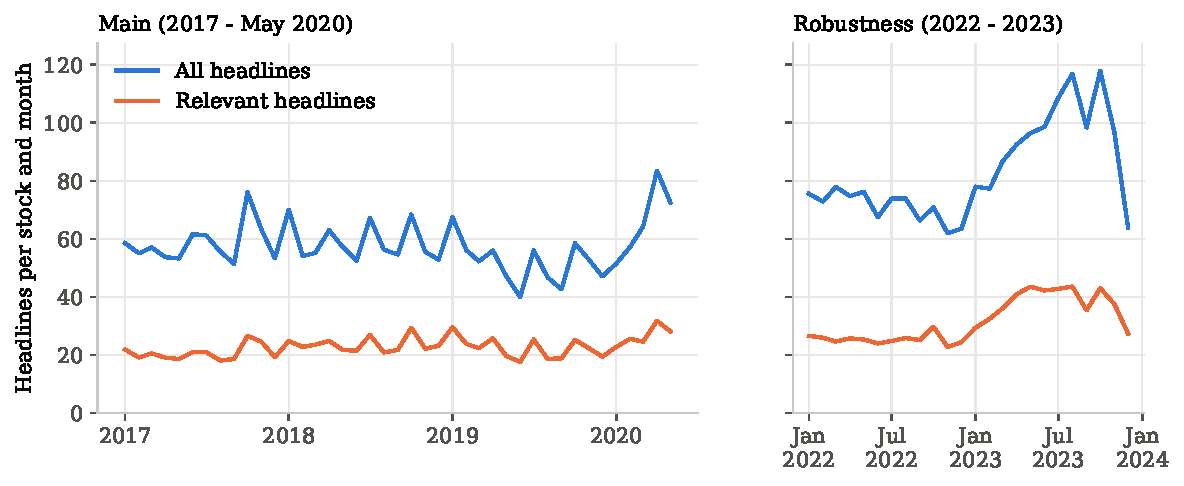
\includegraphics[width=\textwidth]{figure1_news_coverage.pdf}
  \caption[News coverage over time]{News coverage over time: average number of headlines per stock and month, all headlines and relevant headlines.}
  \label{fig:coverage}
\end{figure}

\subsection{FinBERT Scores and Daily News Features}\label{sec:data-features}
Each relevant headline is passed through FinBERT (Section~\ref{sec:finbert-model}), which returns a probability for each of the classes positive, negative and neutral. The sentiment score of a headline is the probability of the positive class minus the probability of the negative class, so it lies between $-1$ and $+1$. The headlines are then aggregated to the level of a stock and a trading day, as described in Section~\ref{sec:features}: the number of relevant headlines $n_{i,t}$, the share of negative headlines $\text{neg}_{i,t}$ and the mean sentiment score $\text{sent}_{i,t}$.

Table~\ref{tab:examples} gives examples of headlines for each FinBERT class. The positive and negative examples are plausible in content: positive headlines refer to earnings above expectations or rising prices, negative headlines to falling prices or risks. The neutral class contains many standardised headlines, for instance daily sector updates that merely list tickers. Such headlines carry a score of almost zero, which is the intended behaviour. It also explains why about two thirds of all headlines are classified as neutral (Table~\ref{tab:news}). The examples were drawn from headlines with a class probability above 0.95 and illustrate the classification; they are not a measure of its accuracy.

\begin{table}[htbp]
  \centering\small
  \caption[Examples of FinBERT classifications]{Examples of headlines with a FinBERT class probability above 0.95. The score is the probability of the positive class minus the probability of the negative class.}
  \label{tab:examples}
  \begin{tabular}{lp{9.2cm}r}
    \toprule
    Label & Headline & Score \\
    \midrule
    Positive & Broadcom Shows Rising Price Performance With Jump To 83 RS Rating & +0.93 \\
    Positive & Citigroup Analyst Says Digital Push Should Lift Operating Profit & +0.93 \\
    Positive & Palo Alto Networks (PANW) Surpasses Q4 Earnings and Revenue Estimates & +0.93 \\
    Negative & Amazon Stock Could Be Hurt by an Emerging Trend & $-$0.96 \\
    Negative & Vistagen Shares Fall Under \$1 After Depression Drug Flunks Midstage Trial & $-$0.95 \\
    Negative & Why Is Deere (DE) Down 1.8\% Since its Last Earnings Report? & $-$0.96 \\
    Neutral & Energy Sector Update for 04/16/2019: BRS, TS, XOM, CVX, COP, SLB, OXY & +0.01 \\
    Neutral & Health Care Sector Update for 01/14/2020: JNJ, PFE, ABT, MRK, AMGN, RTIX, TRXC, MREO & +0.00 \\
    \bottomrule
  \end{tabular}
\end{table}

The three features are related to each other, which matters for the interpretation of the coefficients later. Table~\ref{tab:corr} reports their correlations in the main sample. Across all stock-days, the number of headlines is positively correlated with the share of negative headlines (0.28) and with the sentiment score (0.18). This mostly reflects the fact that tone is only defined on days with news. Restricting the sample to days with at least one relevant headline removes this effect: the correlations with the number of headlines become close to zero (0.07 and 0.00). Tone and sentiment remain strongly and negatively correlated ($-0.57$ on all days and $-0.68$ on days with news), because they are two summaries of the same FinBERT output. The intensity of news is therefore a largely separate source of information, whereas the two tone variables overlap strongly. As a consequence, the individual coefficients of the two tone variables are estimated imprecisely and should be interpreted together and with caution (Section~\ref{sec:results-insample}).

\begin{table}[htbp]
  \centering\small
  \caption[Correlations of the news features]{Correlations of the daily news features, main sample. $n$ is the number of relevant headlines, neg the share of negative headlines and sent the mean sentiment score.}
  \label{tab:corr}
  \begin{tabular}{lrrr}
    \toprule
     & $\log(1+n)$ & neg & sent \\
    \midrule
    \multicolumn{4}{l}{\emph{All stock-days}} \\
    $\log(1+n)$ & 1.00 & 0.28 & 0.18 \\
    neg & 0.28 & 1.00 & $-$0.57 \\
    sent & 0.18 & $-$0.57 & 1.00 \\
    \midrule
    \multicolumn{4}{l}{\emph{Days with at least one relevant headline}} \\
    $\log(1+n)$ & 1.00 & 0.07 & $-$0.00 \\
    neg & 0.07 & 1.00 & $-$0.68 \\
    sent & $-$0.00 & $-$0.68 & 1.00 \\
    \bottomrule
  \end{tabular}
\end{table}

% =====================================================================
\section{Scientific Approach}\label{sec:method}
% =====================================================================

\subsection{Baseline Volatility Models}\label{sec:method-baseline}
All baseline models forecast the conditional variance $\sigma_t^2$ of the return $r_t = \sigma_t z_t$ one day ahead, with a mean of zero and standardised errors $z_t$. The GARCH models are re-estimated at the beginning of every month on all data available up to that point (expanding window). The estimated parameters are then used to produce one-day-ahead forecasts for each day of the month, using the observed returns up to the previous day. Forecasts are therefore always out of sample.

\subsubsection{GARCH(1,1) with Normal Errors}\label{sec:garch-n}
The GARCH(1,1) model of \textcite{bollerslev1986} is given in Equation~\eqref{eq:garch}. With normally distributed errors, the parameters $\omega$, $\alpha$ and $\beta$ are estimated by maximum likelihood. Even if the errors are not normal, the estimates remain consistent under mild conditions, which is known as quasi-maximum likelihood estimation \parencite{bollerslev1992}.

\subsubsection{GARCH(1,1) with Student-t Errors}\label{sec:garch-t}
Daily stock returns have much heavier tails than the normal distribution (Table~\ref{tab:descriptive}). Replacing the normal distribution by a Student-t distribution with $\nu$ degrees of freedom, as proposed by \textcite{bollerslev1987}, accommodates these tails. The variance equation is unchanged, and $\nu$ is estimated together with the other parameters.

\subsubsection{GJR-GARCH(1,1) with Student-t Errors}\label{sec:gjr}
The asymmetric GJR-GARCH model of \textcite{glosten1993} allows negative returns to raise the variance more than positive returns of the same size:
\begin{equation}
  \sigma_t^2 = \omega + \left(\alpha + \gamma\,\mathbf{1}\{\varepsilon_{t-1} < 0\}\right)\varepsilon_{t-1}^2 + \beta\,\sigma_{t-1}^2,
  \label{eq:gjr}
\end{equation}
where $\mathbf{1}\{\cdot\}$ is an indicator function that equals one if the previous return was negative, and $\gamma$ measures the additional effect of negative returns (the leverage effect). Errors follow a Student-t distribution.

\subsubsection{Exponentially Weighted Moving Average}\label{sec:ewma}
The EWMA model of the RiskMetrics framework \parencite{riskmetrics1996} computes the variance recursively as
\begin{equation}
  \sigma_t^2 = \lambda\,\sigma_{t-1}^2 + (1 - \lambda)\,r_{t-1}^2,
  \label{eq:ewma}
\end{equation}
with the standard daily decay factor $\lambda = 0.94$. No parameters are estimated.

\subsubsection{Properties of the Baseline Models}\label{sec:model-properties}
The four baseline models differ in how they treat persistence and asymmetry; Table~\ref{tab:models} summarises the differences. In the GARCH(1,1) model, the sum $\alpha+\beta$ measures the persistence of volatility shocks. If it is below one, variance returns to the long-run level $\omega/(1-\alpha-\beta)$, and the half-life of a shock is $\ln(0.5)/\ln(\alpha+\beta)$ days. Estimates for daily stock returns are typically close to one, which means that volatility shocks die out slowly. The GJR-GARCH model adds the term $\gamma\,\mathbb{1}[r_{t-1}<0]\,r_{t-1}^2$, so that negative returns raise future variance by more than positive returns of the same size (the leverage effect). Its persistence is $\alpha+\gamma/2+\beta$ if the shock distribution is symmetric. The EWMA model of RiskMetrics \parencite{riskmetrics1996} is the special case of an integrated GARCH model with $\omega=0$, $\alpha=1-\lambda$ and $\beta=\lambda$. It has no long-run level to which the variance returns and no parameters that need to be estimated, which makes it robust but also inflexible. These differences are relevant for the results: a model with a long-run level and an asymmetric reaction can adapt better to changing market conditions, while EWMA, which cannot, leaves the most room for an external signal such as news.

\begin{table}[htbp]
  \centering\small
  \caption[Properties of the baseline models]{Properties of the baseline volatility models.}
  \label{tab:models}
  \begin{tabular}{p{2.2cm}p{4.5cm}p{2.4cm}p{2.2cm}p{2.2cm}}
    \toprule
    Model & Variance equation & Error distribution & Asymmetry & Parameters \\
    \midrule
    GARCH-N & $\omega+\alpha r_{t-1}^2+\beta\sigma_{t-1}^2$ & Normal & No & 3 \\
    GARCH-t & $\omega+\alpha r_{t-1}^2+\beta\sigma_{t-1}^2$ & Student-$t$ & No & 4 \\
    GJR-GARCH-t & $\omega+(\alpha+\gamma\mathbb{1}[r_{t-1}<0])r_{t-1}^2+\beta\sigma_{t-1}^2$ & Student-$t$ & Yes & 5 \\
    EWMA & $(1-\lambda)r_{t-1}^2+\lambda\sigma_{t-1}^2$, $\lambda=0.94$ & --- & No & 0 \\
    \bottomrule
  \end{tabular}
\end{table}

\subsection{Sentiment Measurement with FinBERT}\label{sec:method-finbert}
\subsubsection{The FinBERT Model}\label{sec:finbert-model}
FinBERT \parencite{araci2019} is a BERT model \parencite{devlin2019} that has been further pre-trained on financial text and fine-tuned to classify financial sentences as positive, negative or neutral. The publicly available ProsusAI/finbert model is used without any further training. For each headline, the model returns three probabilities. The label order (positive, negative, neutral) was read from the configuration of the model rather than assumed. Headlines were processed on a GPU in batches with a maximum length of 64 tokens, which is sufficient for headlines. The sentiment score of a headline is
\begin{equation}
  s = P(\text{positive}) - P(\text{negative}),
  \label{eq:sentiment}
\end{equation}
which ranges from $-1$ (clearly negative) to $+1$ (clearly positive).

\subsubsection{Feature Engineering and Aggregation}\label{sec:features}
For every stock $i$ and trading day $t$, the relevant headlines assigned to that day by the timing rule (Section~\ref{sec:data-news}) are aggregated to three features:
\begin{itemize}
  \item $n_{i,t}$, the number of relevant headlines, which measures news intensity. It enters the model as $\log(1 + n_{i,t})$ to dampen the influence of days with exceptionally many headlines.
  \item $\text{neg}_{i,t}$, the share of relevant headlines classified as negative.
  \item $\text{sent}_{i,t}$, the average sentiment score of the relevant headlines.
\end{itemize}
On days without relevant news (about half of all stock-days in the main sample), $\text{neg}_{i,t}$ and $\text{sent}_{i,t}$ are set to zero.

\subsection{News-Augmented Forecasts}\label{sec:method-news}
The news-augmented forecast scales the baseline forecast with the news features:
\begin{equation}
  \hat\sigma^2_{\text{news},i,t} = \hat\sigma^2_{\text{base},i,t}\,\exp\!\left(c + b_1 \log(1 + n_{i,t}) + b_2\, \text{neg}_{i,t} + b_3\, \text{sent}_{i,t}\right),
  \label{eq:news-model}
\end{equation}
where $\hat\sigma^2_{\text{base},i,t}$ is the one-day-ahead variance forecast of the baseline model, $c$ is a constant that corrects the general level of the baseline forecast, and $b_1$, $b_2$, $b_3$ are the coefficients of the news features. The exponential form guarantees positive forecasts, and $\exp(b_1\log(1+n)) = (1+n)^{b_1}$ gives the coefficient the interpretation of an elasticity. A positive $b_1$ means that days with more news have a higher variance than the baseline predicts.

The coefficients are estimated by quasi-maximum likelihood (QML), which is the main method. With squared returns $r^2$ as the target, the Gaussian quasi-likelihood leads to minimising the QLIKE loss of the scaled forecast,
\begin{equation}
  \min_{c,\,b}\; \frac{1}{N}\sum_{i,t}\left[\ln \hat\sigma^2_{\text{news},i,t} + \frac{r_{i,t}^2}{\hat\sigma^2_{\text{news},i,t}}\right].
  \label{eq:qml}
\end{equation}
QML is consistent for the conditional variance even if the errors are not normal \parencite{bollerslev1992}, and it uses the same criterion for estimation and evaluation. As a robustness check, the adjustment factor is instead estimated by ordinary least squares (OLS) in a regression of $r_t^2/\hat\sigma^2_{\text{base}}$ on the news features; the fitted factor is bounded below at 0.05 so that forecasts stay positive. The coefficients are pooled across stocks, because individual stocks have too few news days to estimate them reliably. Estimation uses an expanding window that starts at the beginning of the sample window (January 2017 and January 2022) and ends before the forecast month; the coefficients are re-estimated every month. In-sample coefficients over the whole window are reported with standard errors clustered by date, because shocks hit many stocks on the same day.

Several variants are compared:
\begin{itemize}
  \item \emph{Baseline}: the unadjusted forecast of the baseline model.
  \item \emph{Recalibrated baseline}: the baseline multiplied by $\exp(c)$, with $c$ estimated in the same way but without news features. This is the fair benchmark, because any gain of a news model must come from the news and not from a simple correction of the forecast level.
  \item \emph{News intensity}: only $\log(1+n)$ is included.
  \item \emph{News intensity + tone}: all three features are included.
  \item \emph{All headlines (unfiltered)}: the three features are computed from all headlines without the relevance filter.
  \item \emph{Extra one-day lag}: the three features are shifted by one more day. If news mainly carries information that arrives on the same day, this variant should not improve the forecast.
\end{itemize}

\subsubsection{Interpretation and Estimation of the News Adjustment}\label{sec:news-interpretation}
The coefficient $b_1$ can be read as an elasticity. For a coefficient of $b_1=0.4$, a stock-day with one relevant headline has a variance forecast that is higher by a factor of $2^{0.4}\approx 1.32$ than a stock-day without news, and a day with three headlines a factor of $4^{0.4}\approx 1.74$. The effect becomes smaller for each additional headline, which is reasonable because the first headlines of a day are more informative than the tenth. The coefficients $b_2$ and $b_3$ are semi-elasticities: a change of $0.1$ in the share of negative headlines changes the forecast by $100\,(e^{0.1 b_2}-1)$ per cent.

The minimisation in Equation~\eqref{eq:qml} is carried out numerically with the BFGS algorithm. Because the news-adjusted forecast is $\hat\sigma^2_{\text{base}}\exp(x'\theta)$ with $x=(1,\log(1+n),\text{neg},\text{sent})'$, the gradient of the QLIKE loss has a simple closed form,
\begin{equation}
  \frac{\partial}{\partial\theta}\,\frac{1}{N}\sum_{i,t}\text{QLIKE}_{i,t} = \frac{1}{N}\sum_{i,t}\left(1-\frac{r_{i,t}^2}{\hat\sigma^2_{\text{news},i,t}}\right)x_{i,t},
  \label{eq:gradient}
\end{equation}
which is supplied to the optimiser. In every month, the coefficients are re-estimated with all observations up to the end of the previous month, so that the forecast for a day never uses information from that day or later. The first forecast month uses a window of one year of data (2017 for the main sample and 2022 for the robustness sample).

\subsubsection{Why Forecasts Are Compared with the Recalibrated Baseline}\label{sec:method-recal}
A fair test of the news features must separate two things: an improvement that comes from the information in the news, and an improvement that comes only from the fact that the news model has a free constant and can therefore correct the general level of the baseline forecast. Volatility models fitted by maximum likelihood on returns do not necessarily have the right level when the forecasts are evaluated with QLIKE, and the level of the forecast matters for the loss. The recalibrated baseline therefore uses the same estimation procedure as the news model, but only with the constant $c$. A difference between the news model and the recalibrated baseline is attributable to the news features, whereas a difference between the news model and the unadjusted baseline combines both effects. The two comparisons answer different questions, and both are reported (Section~\ref{sec:results-oos}).

\subsection{Forecast Evaluation Methodology}\label{sec:method-evaluation}
\subsubsection{Noisy Proxies and the Choice of Loss Function}\label{sec:method-proxy}
Because the true variance is not observed, forecasts are compared with the squared return. \textcite{andersen1998} show that standard volatility models appear to forecast poorly when judged against squared returns, although the proxy is unbiased, because the proxy is very noisy and most of its variation is unrelated to the variance. The comparison of forecasts is nevertheless valid in the sense that the better forecast has the lower expected loss, but only for some loss functions. \textcite{patton2011} characterises the class of loss functions for which this holds and shows that MSE and QLIKE belong to it, whereas other common losses do not. In practice, the choice between the two matters: MSE gives most weight to the largest errors, and QLIKE is more sensitive to small variances being under-predicted and has a higher power to detect differences between forecasts \parencite{patton2011}. The study of \textcite{hansen2005} compares 330 volatility models and finds that no model clearly beats GARCH(1,1) in an application to exchange rates, although models with a leverage effect are better for stock returns. This result supports the choice of simple GARCH-type benchmarks in the present study.

Forecasts are evaluated against the squared return as the volatility proxy, using two loss functions. The squared-error loss (MSE) is $(r_t^2 - \hat\sigma_t^2)^2$, and the QLIKE loss \parencite{patton2011} is
\begin{equation}
  \text{QLIKE}_t = \ln \hat\sigma_t^2 + \frac{r_t^2}{\hat\sigma_t^2}.
  \label{eq:qlike}
\end{equation}
\textcite{patton2011} shows that both are robust to noise in the proxy, in the sense that they rank forecasts correctly in expectation. QLIKE penalises under-prediction of variance more than over-prediction and is much less affected by extreme observations than MSE. It is therefore the main criterion; MSE, in contrast, is dominated by a few extreme days in the COVID-19 crash.

\subsubsection{Testing Differences in Accuracy}\label{sec:method-dm}
Differences in accuracy are tested with the Diebold--Mariano test \parencite{diebold1995}. For each trading day, the QLIKE loss is averaged across stocks, and the difference between two forecasts is regressed on a constant. The p-value of the constant is based on Newey--West standard errors with five lags \parencite{newey1987}, which accounts for autocorrelation in the loss differences. Averaging across stocks first accounts for correlation of the losses between stocks on the same day. All p-values are two-sided. The news models are tested both against the baseline and against the recalibrated baseline.

% =====================================================================
\section{Results}\label{sec:results}
% =====================================================================

\subsection{Baseline Model Performance}\label{sec:results-baseline}
Table~\ref{tab:baseline} reports the out-of-sample accuracy of the four baseline models. In the main sample (January 2018 to May 2020), the ranking by QLIKE is clear: GJR-GARCH with Student-t errors is the most accurate (2.185), followed by GARCH-t (2.212), GARCH-N (2.223) and EWMA (2.280). The same order holds for MSE. The asymmetric model benefits from the leverage effect, which was pronounced in the sharp decline of February and March 2020. This is in line with H1 and with the finding of \textcite{hansen2005} that models with a leverage effect do better for equity returns.

In the calmer robustness sample (2023), the models are much closer. QLIKE ranges from 1.997 (GJR-t) to 2.002 (GARCH-t), with only EWMA clearly weaker (2.034). For MSE, GARCH-N is marginally best (116.97), and the differences between the three GARCH models are tiny. Where volatility is stable, the choice between GARCH variants hardly matters.

\thesistable{table3_baseline_accuracy}{Out-of-sample accuracy of the baseline models (lower is better). Evaluation periods: January 2018 -- May 2020 (main) and 2023 (robustness).}{tab:baseline}

\subsection{News and Volatility}\label{sec:results-insample}
Figure~\ref{fig:volume} shows the relationship between news volume and volatility without any model. The bars give the mean ratio of the squared return to the GJR-GARCH-t forecast, by the number of relevant headlines on the previous day. If the forecast were unbiased and unrelated to news, the ratio would be one in every group. On days without relevant news the ratio is 0.90, with one headline it is 0.99, with two or three headlines 1.19, and with four or more headlines 2.30. Days with many headlines are therefore days on which realised variance is more than twice the level that the price-based model expects.

\begin{figure}[htbp]
  \centering
  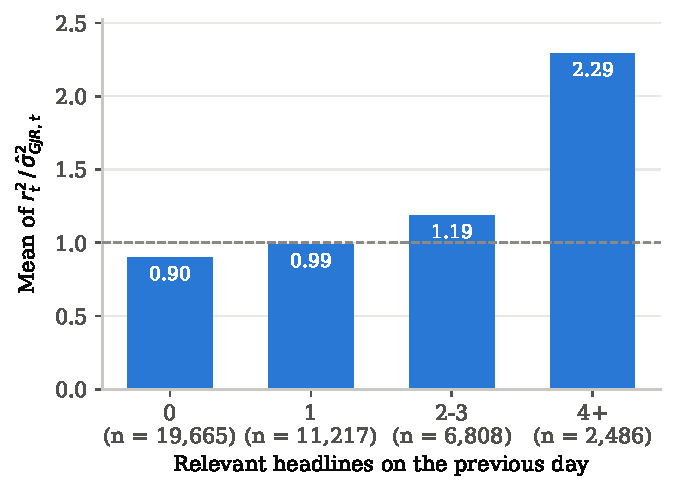
\includegraphics[width=0.65\textwidth]{figure2_news_volume_vs_volatility.pdf}
  \caption[Squared returns relative to the GARCH forecast by news volume]{Mean ratio of the squared return to the GJR-GARCH-t forecast, by the number of relevant headlines on the previous day (main sample, January 2017 -- May 2020).}
  \label{fig:volume}
\end{figure}

Table~\ref{tab:coefficients} reports the estimates of Equation~\eqref{eq:news-model} over the whole sample window. The coefficient of news intensity is 0.434 in the main sample (t-statistic 12.9). This means that a single relevant headline raises the expected variance by a factor of $2^{0.434} \approx 1.35$, i.e.\ by about 35\%, and four headlines by a factor of $5^{0.434} \approx 2.0$. In the robustness sample, the coefficient is 0.267 (t-statistic 6.2), corresponding to an increase of about 20\% for one headline. News intensity is thus strongly related to variance in both samples, which supports H2.

The tone features are less clear. In the main sample, the coefficient of the average sentiment is $-0.413$ (t-statistic $-6.6$), so more positive news goes together with lower variance, as expected. The coefficient of the share of negative headlines is $-0.418$ (t-statistic $-2.6$), which has the opposite sign from what one would expect from negative news on its own. The two features are strongly correlated, so their individual coefficients should not be interpreted separately; their joint effect is what matters. In the robustness sample, neither tone coefficient is significantly different from zero. Tone therefore does not add a stable explanation of variance, and the effect operates mainly through the volume of news.

\thesistable{table5_news_coefficients}{In-sample estimates of the news adjustment in Equation~\eqref{eq:news-model} for the GJR-GARCH-t baseline, quasi-maximum likelihood, whole sample windows (main: January 2017 -- May 2020; robustness: 2022--2023). Standard errors are clustered by date.}{tab:coefficients}

\subsection{Out-of-Sample Forecast Accuracy}\label{sec:results-oos}
Table~\ref{tab:news-gjr} reports the main out-of-sample result for the best baseline, GJR-GARCH-t. The recalibrated baseline is not better than the baseline (2.188 versus 2.185 in the main sample), so recalibration alone brings no benefit, and the comparison with it isolates the contribution of the news.

Both news variants improve on the recalibrated baseline. With news intensity only, QLIKE falls to 2.172 in the main sample and 1.984 in the robustness sample; adding tone gives 2.170 and 1.986. The differences from the recalibrated baseline are statistically significant at the 5\% level in both samples (p = 0.050 and 0.035 in the main sample, p = 0.024 and 0.038 in the robustness sample). Against the untouched baseline, the improvement is of the same size but the p-values are above 5\% (0.123 and 0.085 in the main sample, 0.240 and 0.290 in the robustness sample). The gain is small: 0.015 QLIKE points in the main sample, about 0.7\% of the loss. Section~\ref{sec:discussion} discusses whether this is economically meaningful.

The \emph{extra lag} variant shows that the information is short-lived. When the news features are shifted by one more day, QLIKE (2.189 and 2.001) is no better than the baseline, and the p-values against the recalibrated baseline are 0.77 and 0.70. It is the news of the preceding day, not older news, that carries the information.

Figure~\ref{fig:cumulative} shows when the gains occur. In the main sample, the news model improves on the recalibrated baseline on average during 2018 and 2019 and in the weeks of January and mid-February 2020. From about 20 February 2020, when the market collapsed, the news model becomes worse than the recalibrated baseline: the mean daily QLIKE difference is $-0.026$ in 2018--2019 and $-0.037$ in January to mid-February 2020, but $+0.042$ from 20 February 2020 until the end of the sample. Over the whole evaluation period the news model is better on 56\% of days, and its average QLIKE is lower than that of the recalibrated baseline for 27 of the 47 stocks.

\thesistable{table4_news_models_gjr}{Out-of-sample accuracy of news-augmented forecasts, GJR-GARCH-t baseline, quasi-maximum likelihood estimation. Evaluation periods: January 2018 -- May 2020 (main sample) and 2023 (robustness sample). p-values from Diebold--Mariano tests on QLIKE against the baseline and the recalibrated baseline (Newey--West standard errors, 5 lags).}{tab:news-gjr}

\begin{figure}[htbp]
  \centering
  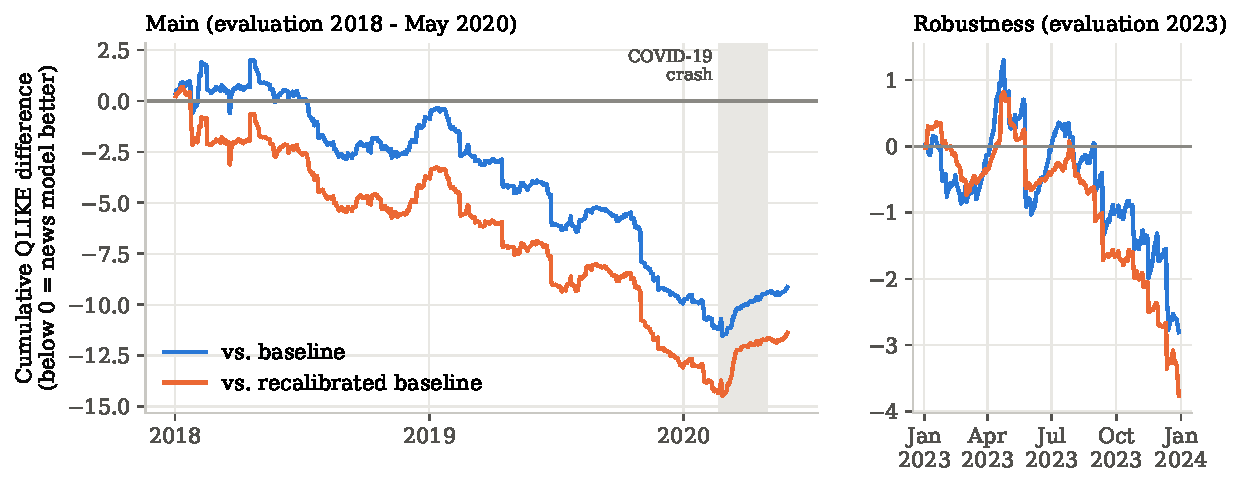
\includegraphics[width=\textwidth]{figure3_cumulative_qlike_gain.pdf}
  \caption[Cumulative QLIKE difference of the news-augmented model]{Cumulative difference in daily QLIKE loss between the news-augmented GJR-GARCH-t model (news intensity and tone) and the baselines. Values below zero indicate that the news model is more accurate.}
  \label{fig:cumulative}
\end{figure}

\subsection{Accuracy Across Periods and Stocks}\label{sec:results-periods}
\subsubsection{Sub-Periods}\label{sec:results-subperiods}
Table~\ref{tab:subperiods} splits the evaluation period into sub-periods and reports the mean daily QLIKE of the GJR-GARCH-t baseline, of the recalibrated baseline and of the news model with intensity and tone. In the main sample, the news model is more accurate than the recalibrated baseline in both full years (by 0.015 in 2018 and 0.037 in 2019) and in the weeks before the crash (by 0.037). In 2019, it is better on 63\% of the days. In the crash period from 20 February 2020 the picture reverses: the news model is less accurate by 0.042 and better on only 33\% of the days. The average loss of all models is about twice as high in this period (around 3.95 against 1.7 to 2.1 in the other periods).

In the robustness sample, the news model is more accurate than the recalibrated baseline in each quarter of 2023, but the differences are small in the first half of the year (0.006 and 0.001) and larger in the second half (0.020 and 0.033). The share of days on which the news model is better is below 50\% in three of the four quarters. The result for 2023 as a whole therefore rests on a modest improvement on many days and a larger improvement on some.

\begin{table}[htbp]
  \centering\small
  \caption[Out-of-sample QLIKE by sub-period]{Mean daily QLIKE by sub-period, GJR-GARCH-t baseline, news model with intensity and tone (QML). The column \enquote{News $-$ recal.} is the difference to the recalibrated baseline; negative values favour the news model. The last column is the share of days on which the news model has the lower loss.}
  \label{tab:subperiods}
  \begin{adjustbox}{max width=\textwidth}
  \begin{tabular}{lrrrrrr}
    \toprule
    Period & Days & Baseline & Recal. & News & News $-$ recal. & Days news better (\%) \\
    \midrule
    2018 & 251 & 2.109 & 2.121 & 2.106 & $-$0.015 & 55 \\
    2019 & 252 & 1.822 & 1.823 & 1.786 & $-$0.037 & 63 \\
    1 Jan -- 19 Feb 2020 & 33 & 1.751 & 1.750 & 1.713 & $-$0.037 & 55 \\
    20 Feb -- 31 May 2020 (crash) & 70 & 3.966 & 3.954 & 3.996 & +0.042 & 33 \\
    \midrule
    2023 Q1 & 62 & 2.140 & 2.144 & 2.138 & $-$0.006 & 47 \\
    2023 Q2 & 62 & 2.032 & 2.035 & 2.034 & $-$0.001 & 37 \\
    2023 Q3 & 63 & 1.883 & 1.887 & 1.868 & $-$0.020 & 49 \\
    2023 Q4 & 63 & 1.936 & 1.940 & 1.907 & $-$0.033 & 54 \\
    \bottomrule
  \end{tabular}
  \end{adjustbox}
\end{table}

\subsubsection{Individual Stocks}\label{sec:results-stocks}
The pooled coefficients are applied to all stocks alike, so the gains need not be equally distributed. Tables~\ref{tab:app-stock-oos} and \ref{tab:app-stock-oos-rob} in the appendix report the mean QLIKE for each stock. In the main sample, the news model is more accurate than the recalibrated baseline for 27 of the 47 stocks, in the robustness sample for 30 of the 44 stocks. The largest improvements in the main sample are found for Arista Networks (ANET, $-0.277$), Texas Instruments (TXN, $-0.158$), AbbVie (ABBV, $-0.144$), Palo Alto Networks (PANW, $-0.133$) and Oracle (ORCL, $-0.123$). The model is clearly worse for Philip Morris (PM, $+0.171$) and Johnson \& Johnson (JNJ, $+0.108$). The average over all stocks therefore hides a wide spread: gains are concentrated in a minority of stocks, and for a large part of the stocks (20 of 47 in the main sample) the news model does not help.

The gain of a stock can also be related to its average news intensity, measured as the number of relevant headlines per stock-day. In the main sample, the correlation between the two is $-0.29$: stocks with more relevant headlines per day tend to gain more from the news adjustment (a more negative QLIKE difference). In the robustness sample, there is no relationship (correlation $0.07$). The pattern in the main sample is plausible, because the adjustment works through the number of headlines, but its absence in the second sample, together with the small number of stocks, means that it should not be over-interpreted.

\subsubsection{Squared-Error Loss}\label{sec:results-mse}
The conclusions above are based on QLIKE. Table~\ref{tab:mse} shows that the picture is different under the squared-error loss. The news models have a higher MSE than the baseline in both samples (383.9 against 373.2 in the main sample and 122.8 against 117.2 in the robustness sample for the model with intensity and tone), and the recalibrated baseline is also not better than the baseline. The reason lies in how the two loss functions treat extreme days. In the main sample, the 70 crash days account for 70\% of the sum of the daily MSE of the baseline, and the days with the largest losses are 16, 9, 24 and 12 March 2020 and 1 November 2019. MSE is therefore dominated by a handful of extreme observations, and an adjustment that raises forecasts on days with many headlines is penalised heavily if the return on such a day turns out to be small. QLIKE grows less quickly with the size of the error and is the preferred criterion in the literature \parencite{patton2011}, but the result shows that the benefit of the news features depends on the loss function and cannot be claimed in general.

\begin{table}[htbp]
  \centering\small
  \caption[Accuracy of the news models under MSE and QLIKE]{Out-of-sample accuracy of the news-augmented forecasts under the squared-error loss (MSE) and QLIKE, GJR-GARCH-t baseline, QML estimation.}
  \label{tab:mse}
  \begin{adjustbox}{max width=\textwidth}
  \begin{tabular}{lrrrr}
    \toprule
     & MSE (main) & QLIKE (main) & MSE (robust.) & QLIKE (robust.) \\
    \midrule
    Baseline & 373.2 & 2.185 & 117.2 & 1.997 \\
    Recalibrated baseline & 373.9 & 2.188 & 119.4 & 2.001 \\
    News intensity & 382.8 & 2.172 & 122.6 & 1.984 \\
    News intensity + tone & 383.9 & 2.170 & 122.8 & 1.986 \\
    All headlines (unfiltered) & 378.5 & 2.171 & 122.4 & 1.984 \\
    Extra one-day lag & 378.1 & 2.189 & 120.4 & 2.001 \\
    \bottomrule
  \end{tabular}
  \end{adjustbox}
\end{table}

\subsection{Robustness Analysis}\label{sec:results-robustness}
\subsubsection{Relevance Filter}\label{sec:rob-filter}
The variant with unfiltered headlines performs as well as the filtered ones, and slightly better in some respects (QLIKE 2.171 and 1.984; p = 0.007 and 0.002 against the recalibrated baseline). The relevance filter, which removes about 60\% of the headlines, therefore does not improve the forecasts. A plausible reason is that headlines which merely mention other companies or the market still indicate that the stock is in the news; the filter is nevertheless useful for the interpretation of the features, because it ensures that the news concerns the company.

\subsubsection{Estimation Method}\label{sec:rob-ols}
The results depend on the estimation method. With OLS instead of QML (Appendix, Table~\ref{tab:app-GJR-t-ols}), the news models do not beat the baseline in the main sample (QLIKE 2.191 and 2.187 versus 2.185; p = 0.81 and 0.88 against the recalibrated baseline). In the robustness sample, the OLS variants are better than the baseline (1.987 and 1.988), but only the unfiltered variant is significant against the recalibrated baseline (p = 0.006). OLS minimises squared errors on squared returns, which are dominated by extreme days, whereas QML uses the same criterion as the evaluation. The significant gains therefore hold for a well-matched estimator, not for any estimator.

\subsubsection{Alternative Baseline Models}\label{sec:rob-baselines}
The appendix reports the same analysis for the other three baselines (Tables~\ref{tab:app-EWMA-qml} to \ref{tab:app-GARCH-t-qml}) and for OLS estimation (Tables~\ref{tab:app-EWMA-ols} to \ref{tab:app-GARCH-t-ols}). The pattern is similar but the strength differs. The gains are largest for the weakest baseline: for EWMA, the news models reduce QLIKE from 2.280 to 2.228--2.233 in the main sample, and the improvement is significant against both the baseline and the recalibrated baseline (p $\leq$ 0.022). Even then, the improved EWMA remains less accurate than the plain GJR-GARCH-t baseline (2.185). For the two plain GARCH models, the improvement over the recalibrated baseline is smaller and in the main sample only significant for the unfiltered variant of GARCH-t (p = 0.025); in the robustness sample, the unfiltered variants (p = 0.007 and 0.009) and the intensity-only variant of GARCH-N (p = 0.036) are significant against the recalibrated baseline, while the other variants are not (p between 0.054 and 0.086). News features thus help most where the benchmark is weakest, and the results are most stable for the QML estimator.

\subsubsection{A Closer Look at One Stock}\label{sec:rob-example}
Figure~\ref{fig:example} shows the forecasts for one stock, Gilead Sciences, during the COVID-19 crash. It illustrates the forecasts of the GJR-GARCH-t model with and without the news adjustment around the sharpest phase of the crash, and shows that the news adjustment is a modification of the baseline forecast and not a separate model.

\begin{figure}[htbp]
  \centering
  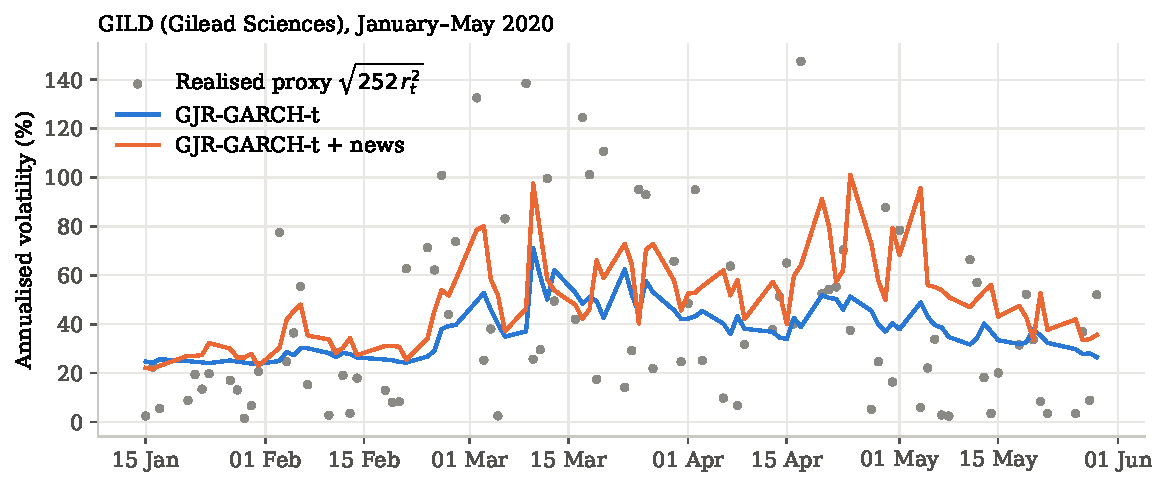
\includegraphics[width=\textwidth]{figure4_example_gild.pdf}
  \caption[Forecasts for Gilead Sciences during the COVID-19 crash]{Gilead Sciences (GILD), January -- May 2020: realised volatility proxy and forecasts of the GJR-GARCH-t model with and without news.}
  \label{fig:example}
\end{figure}

% =====================================================================
\section{Discussion}\label{sec:discussion}
% =====================================================================

\subsection{Interpretation of Baseline Results}\label{sec:disc-baseline}
The ranking of the baseline models confirms the view that carefully specified GARCH models are difficult to improve. The advantage of the GJR specification in the main sample is explained by the leverage effect: negative returns are followed by a stronger increase in variance, which was exactly the pattern of the COVID-19 crash. EWMA, which imposes that shocks never die out and uses a fixed decay, is the least accurate in both samples. The small differences in the calm 2023 sample show that model choice matters most when markets are under stress, and that gains from additional information cannot be large when even the choice between rival models hardly matters.

\subsection{Interpretation of Enhanced Model Results}\label{sec:disc-enhanced}
The central finding is that the volume of company-specific news is associated with higher variance, and that this relationship can be used to improve forecasts slightly. News intensity can be understood as a measure of investor attention: the more a company is in the news, the more investors trade and revise their views, which leads to larger price changes \parencite{barber2008}. This explanation is consistent with the fact that tone adds little. A possible reason is that the direction of the news is priced quickly, while the fact that something is happening raises uncertainty regardless of direction. For volatility, in contrast to returns, the arrival of information matters more than its sign.

The short life of the effect is equally important. When the news features are lagged by one additional day, the gain disappears completely. Markets incorporate news into prices within a day, so that news carries information about volatility mainly on the day it appears.

The gains are not stable over time. The news model helps in calm and moderately turbulent periods and loses in the sharpest phase of the COVID-19 crash. A possible explanation is that the coefficient is estimated on pre-crisis data, in which a high number of headlines signalled a company-specific event. In the crash, volatility was driven by a market-wide shock that affected all stocks regardless of how many headlines each had, so the company-specific news signal was no longer informative about the size of the move. The coefficients estimated on calm data then add noise instead of information. This is a hypothesis; the available data cannot separate it from other explanations.

The size of the gains also depends on the benchmark. News features help most where the benchmark is weakest (EWMA) and least where it is strongest (GJR-GARCH-t), and a news-augmented EWMA is still less accurate than the plain GJR-GARCH-t. Choosing a good price-based model is therefore more important than adding news.

\subsection{Comparison with Related Literature}\label{sec:disc-literature}
The results are consistent with the evidence that text contains information about future risk that is not in past prices. \textcite{glasserman2019} find that unusual news predicts higher volatility, and the positive and significant effect of news intensity in this thesis points in the same direction, although the measure is simpler (a count of relevant headlines) and the horizon is one day. The finding that sentiment adds little qualifies the message of \textcite{tetlock2007} and \textcite{loughran2011} that the tone of news is informative: for volatility, the tone of short headlines is a weaker signal than the amount of news. The thesis also confirms the message of \textcite{hansen2005} that strong benchmarks leave little room for improvement: the best news model reduces the loss by less than one percent.

The thesis differs from studies of language models for return prediction \parencite{lopezlira2023} in an important respect. Return prediction asks for the direction of price changes and relies on sentiment. Volatility forecasting asks for the size of price changes, and the main source of information here is the amount of news. This distinction may explain why FinBERT, whose output is used as a measure of tone, contributes less than the simple count of headlines.

\subsection{Assessment of the Hypotheses}\label{sec:disc-hypotheses}
Table~\ref{tab:hypotheses} summarises how the evidence relates to the three hypotheses of Section~\ref{sec:rq}. H1 and H2 are supported. H3 is supported only in a restricted sense: the improvement over the recalibrated baseline is statistically significant for the best baseline and for EWMA, but it is small, it depends on the estimation method and the loss function, and it is limited to the first day after the news.

\begin{table}[htbp]
  \centering\small
  \caption[Assessment of the hypotheses]{Assessment of the hypotheses.}
  \label{tab:hypotheses}
  \begin{tabular}{p{2.8cm}p{6.0cm}p{3.4cm}}
    \toprule
    Hypothesis & Evidence & Assessment \\
    \midrule
    H1: strong benchmark, GJR-GARCH-t best & GJR-t has the lowest QLIKE and MSE in the main sample; the GARCH models are almost tied in 2023; EWMA is the weakest in both samples & Supported \\
    H2: news is related to higher variance & News intensity has a significant positive coefficient in both samples; tone is significant only in the main sample & Supported for news intensity; tone not robust \\
    H3: news improves out-of-sample forecasts & QLIKE falls by less than 1\% in both samples; significant against the recalibrated baseline, not against the baseline; no gain with an extra lag; higher MSE; no gain with OLS in the main sample; reversal in the crash & Partly supported \\
    \bottomrule
  \end{tabular}
\end{table}

\subsection{Threats to Validity}\label{sec:disc-validity}
Several features of the design limit how far the results can be generalised, and they are listed here because they affect how the small improvements in forecast accuracy should be read.

\emph{Selection of well-covered stocks.} The stocks were selected because the dataset contains a continuous flow of headlines about them. This is necessary to distinguish days without news from gaps in the data, but it means that the sample is not a random draw of large companies. Companies with a continuous news record may be more heavily followed by the press and by investors, and the effect of news on volatility may be different for companies that are covered less often. Several of the largest companies are absent from the main sample for this reason.

\emph{Daily dates without a time of day.} Because headlines carry no reliable time stamp, every headline is assigned to the next trading day. This avoids look-ahead bias, but it also means that information published during the trading day is only used with a delay of up to one day. If the true effect of news is concentrated within a few hours, the design underestimates it. The lack of improvement from an additional lag (Table~\ref{tab:mse}) is consistent with this reading: the information in news is short-lived.

\emph{Noise in tags and sentiment.} The ticker tags of FNSPID are noisy, and the relevance filter, although it agrees with the manual labels in 98 of 100 cases, is a rule based on names and symbols. FinBERT was trained on financial text, but it classifies headlines without knowing the context, and most headlines are neutral. Part of the signal in the tone variables may therefore be lost, which is another possible reason for the weak and unstable tone coefficients.

\emph{Pooled coefficients.} The news coefficients are the same for all stocks. This is a restriction that makes the estimation feasible, but the results by stock (Section~\ref{sec:results-stocks}) show that the effect is not the same for all stocks. A model with coefficients that depend on characteristics of the stock, for example its size or its news intensity, might perform better, but it would also need more data.

\emph{Proxy and multiple comparisons.} The squared return is a noisy proxy for the variance, which makes the loss differences small relative to the day-to-day variation of the losses. The analysis compares several baselines, several news variants and two samples, and each comparison is a separate test. A significant result in one of them is not strong evidence on its own, which is why the conclusions are based on the pattern across variants and samples, and not on a single p-value.

\emph{Two regimes.} The main sample ends in the middle of the COVID-19 crash, and the robustness sample covers a different period with different news intensity. Both are periods of high uncertainty in markets. The results may differ in a calm market in which volatility is low and changes slowly.

\subsection{Practical Implications}\label{sec:disc-practical}
For practitioners, the results suggest a cautious conclusion. News features can be added cheaply to a GARCH model, they improve the forecasts modestly in normal times, and they should be re-estimated regularly. They should not be relied on in crises, where they may mislead. A gain of less than one percent in QLIKE is unlikely to change a trading or hedging decision on its own, but it may be worthwhile for a risk manager who already has news data available and who runs forecasts for many stocks. More sophisticated language models should only be considered if they extract information that a simple headline count does not.

\subsection{Limitations}\label{sec:disc-limitations}
Several limitations should be kept in mind.
\begin{itemize}
  \item \emph{Data.} FNSPID has coverage gaps, and only about 40\% of the headlines name the company they are tagged to. Timestamps are available at the daily level only, so intraday reactions cannot be analysed and the timing rule is conservative. Headlines are short and cannot reflect the content of full articles.
  \item \emph{Sample.} The candidates were ranked by current market capitalisation and then selected on the basis of news coverage. Companies that are large today are those that grew successfully, which introduces survivorship bias and limits generalisation to smaller firms. The main sample contains one extreme episode, the COVID-19 crash, which has a large influence on the results.
  \item \emph{Volatility proxy.} Squared returns are an unbiased but noisy proxy for the variance. Realised volatility from high-frequency data would give a more precise benchmark.
  \item \emph{Estimation.} The results depend on the estimation method: they hold for QML but not for OLS. Coefficients are pooled across stocks and assumed to be constant, which may not hold across firms or regimes.
  \item \emph{Multiple comparisons.} Several baselines, variants and samples are compared. The p-values, which are close to 5\%, are not adjusted for multiple testing, and the evidence for forecast gains should therefore be seen as suggestive rather than conclusive.
  \item \emph{Language model.} Only one model, FinBERT, was used, without fine-tuning on the volatility task. Results for larger or fine-tuned models may differ.
\end{itemize}

% =====================================================================
\section{Conclusion}\label{sec:conclusion}
% =====================================================================

\subsection{Summary of Contributions}\label{sec:conclusion-summary}
This thesis asked whether news features extracted with the financial language model FinBERT improve one-day-ahead volatility forecasts of large US stocks beyond GARCH-type and EWMA benchmarks. Using 47 stocks from 2017 to May 2020 and 44 stocks in 2022--2023, the analysis found that the GJR-GARCH model with Student-t errors is the best baseline (H1), that news intensity is strongly and positively related to variance (H2), and that, for this baseline, news-augmented forecasts are slightly but significantly better than a recalibrated baseline (H3). The gains are small, depend on the estimation method, last for one day only and reverse during the sharpest phase of the COVID-19 crash. Tone adds little to intensity, and a relevance filter does not improve the forecasts.

The contribution of the thesis is a transparent, reproducible pipeline and a realistic assessment: language-model news features carry some information about volatility, but a large part of it is already contained in a simple count of headlines and the benchmark is hard to beat.

\subsection{Implications for Theory and Practice}\label{sec:conclusion-implications}
For theory, the results support the view that news affects volatility through attention and the arrival of information rather than through direction, and that this effect is quickly absorbed. For practice, they suggest that news features may be a cheap addition to existing risk models in normal times, but not a substitute for well-specified price-based models and not a safeguard in crises.

\subsection{Future Research Directions}\label{sec:conclusion-future}
Several extensions follow from the limitations. Intraday timestamps would allow the timing of news to be measured exactly and the speed of the reaction to be studied. Realised volatility from high-frequency data would provide a more precise benchmark than squared returns. The news adjustment could be made regime-dependent so that it adapts in crises. Larger or fine-tuned language models, and models that read full articles instead of headlines, could be tested to see whether they contain information beyond intensity. Finally, applying the approach to other markets and to smaller firms would show how far the results generalise.

% =====================================================================
%  References
% =====================================================================
\newpage
\printbibliography[heading=bibintoc,title={References}]

% =====================================================================
%  Appendix
% =====================================================================
\newpage
\appendix
\section{Appendix}\label{sec:appendix}

\subsection{List of Stocks Analysed}\label{sec:appendix-stocks}
Main sample (47 stocks): ABBV, ABT, ACN, ADI, AMAT, AMD, AMGN, ANET, APH, AVGO, AXP, BAC, BLK, C, CAT, COP, COST, CRM, CVX, DE, DHR, GE, GILD, GS, HD, JNJ, KO, MRK, MS, MU, NEE, NFLX, NVDA, ORCL, PANW, PEP, PFE, PM, QCOM, T, TJX, TMO, TMUS, TXN, UNP, V, WFC.

Robustness sample (44 stocks): ABBV, ABT, ACN, ADI, AMAT, AMD, AMGN, ANET, CAT, COP, COST, CRM, CRWD, CVX, DE, DELL, DHR, DIS, GE, GILD, GOOG, GS, INTC, KO, MRK, MS, MU, NEE, NVDA, ORCL, PANW, PEP, PM, QCOM, T, TJX, TMO, TMUS, TXN, UNP, V, WFC, WMT, XOM.

\subsection{News-Augmented Forecasts for All Baseline Models}\label{sec:appendix-tables}
\thesistable{tableA_news_models_EWMA_QML}{News-augmented forecasts, EWMA baseline, quasi-maximum likelihood. Columns as in Table~\ref{tab:news-gjr}.}{tab:app-EWMA-qml}
\thesistable{tableA_news_models_GARCH-N_QML}{News-augmented forecasts, GARCH-N baseline, quasi-maximum likelihood. Columns as in Table~\ref{tab:news-gjr}.}{tab:app-GARCH-N-qml}
\thesistable{tableA_news_models_GARCH-t_QML}{News-augmented forecasts, GARCH-t baseline, quasi-maximum likelihood. Columns as in Table~\ref{tab:news-gjr}.}{tab:app-GARCH-t-qml}
\thesistable{tableA_news_models_GJR-t_QML}{News-augmented forecasts, GJR-t baseline, quasi-maximum likelihood. Columns as in Table~\ref{tab:news-gjr}.}{tab:app-GJR-t-qml}

\subsection{Robustness: Ordinary Least Squares Estimation}\label{sec:appendix-ols}
\thesistable{tableA_news_models_EWMA_OLS}{News-augmented forecasts, EWMA baseline, ordinary least squares (robustness). Columns as in Table~\ref{tab:news-gjr}.}{tab:app-EWMA-ols}
\thesistable{tableA_news_models_GARCH-N_OLS}{News-augmented forecasts, GARCH-N baseline, ordinary least squares (robustness). Columns as in Table~\ref{tab:news-gjr}.}{tab:app-GARCH-N-ols}
\thesistable{tableA_news_models_GARCH-t_OLS}{News-augmented forecasts, GARCH-t baseline, ordinary least squares (robustness). Columns as in Table~\ref{tab:news-gjr}.}{tab:app-GARCH-t-ols}
\thesistable{tableA_news_models_GJR-t_OLS}{News-augmented forecasts, GJR-t baseline, ordinary least squares (robustness). Columns as in Table~\ref{tab:news-gjr}.}{tab:app-GJR-t-ols}

\subsection{Data by Stock}\label{sec:appendix-bystock}
\begingroup\small\setlength{\tabcolsep}{4pt}
Tables~\ref{tab:app-stock-desc} to \ref{tab:app-stock-news-rob} report the return and news data for each stock. They show the heterogeneity behind the averages in Section~\ref{sec:data}: annualised volatility in the main sample ranges from 21\% (Coca-Cola) to 60\% (AMD), and the number of relevant headlines per stock-day from 0.40 (Amphenol) to 2.65 (Gilead Sciences).

\begin{longtable}{lrrrrrrr}
\caption[Descriptive statistics by stock]{Descriptive statistics of daily log returns (\%) for each stock, main sample (January 2017 -- May 2020, 857 trading days).}\label{tab:app-stock-desc}\\
\toprule
Stock & Mean & Std.\ dev. & Ann.\ vol. & Min & Max & Skew. & Ex.\ kurt. \\
\midrule
\endfirsthead
\toprule
Stock & Mean & Std.\ dev. & Ann.\ vol. & Min & Max & Skew. & Ex.\ kurt. \\
\midrule
\endhead
\bottomrule
\endfoot
ABBV & 0.064 & 1.94 & 30.7 & -17.7 & 12.9 & -1.36 & 17.2 \\
ABT & 0.113 & 1.60 & 25.5 & -10.3 & 10.4 & -0.12 & 8.5 \\
ACN & 0.070 & 1.63 & 25.8 & -8.8 & 12.1 & 0.15 & 10.1 \\
ADI & 0.060 & 2.18 & 34.6 & -18.2 & 13.7 & -0.58 & 12.0 \\
AMAT & 0.071 & 2.73 & 43.4 & -22.8 & 12.1 & -0.86 & 8.9 \\
AMD & 0.182 & 3.80 & 60.3 & -27.7 & 18.2 & -0.40 & 6.0 \\
AMGN & 0.064 & 1.64 & 26.0 & -8.6 & 10.3 & 0.29 & 6.5 \\
ANET & 0.103 & 2.98 & 47.3 & -27.8 & 17.8 & -1.24 & 16.0 \\
APH & 0.046 & 1.65 & 26.3 & -14.9 & 9.6 & -1.19 & 14.2 \\
AVGO & 0.072 & 2.41 & 38.2 & -22.2 & 14.7 & -1.38 & 16.0 \\
AXP & 0.035 & 2.16 & 34.2 & -16.0 & 19.8 & 0.49 & 23.9 \\
BAC & 0.018 & 2.18 & 34.6 & -16.7 & 16.4 & -0.22 & 14.9 \\
BLK & 0.048 & 1.95 & 31.0 & -14.7 & 12.7 & -0.47 & 11.9 \\
C & -0.016 & 2.38 & 37.8 & -21.4 & 16.5 & -0.84 & 19.2 \\
CAT & 0.041 & 2.05 & 32.6 & -15.4 & 9.8 & -0.73 & 6.5 \\
COP & -0.011 & 2.63 & 41.7 & -28.6 & 22.5 & -1.13 & 28.9 \\
COST & 0.085 & 1.43 & 22.7 & -9.0 & 9.5 & -0.13 & 9.1 \\
CRM & 0.109 & 2.02 & 32.0 & -17.3 & 9.8 & -0.88 & 10.0 \\
CVX & -0.013 & 2.16 & 34.3 & -25.0 & 20.5 & -1.85 & 41.5 \\
DE & 0.053 & 2.05 & 32.5 & -14.6 & 12.5 & -0.59 & 8.0 \\
DHR & 0.091 & 1.46 & 23.2 & -10.2 & 9.3 & -0.00 & 9.2 \\
GE & -0.171 & 2.71 & 43.0 & -16.4 & 13.7 & -0.08 & 6.0 \\
GILD & 0.022 & 1.78 & 28.3 & -9.0 & 9.3 & 0.05 & 4.7 \\
GS & -0.016 & 2.06 & 32.6 & -13.6 & 16.2 & -0.10 & 13.7 \\
HD & 0.081 & 1.78 & 28.2 & -22.1 & 12.9 & -2.28 & 36.1 \\
JNJ & 0.041 & 1.38 & 21.8 & -10.6 & 7.7 & -0.68 & 11.6 \\
KO & 0.026 & 1.32 & 21.0 & -10.2 & 6.3 & -1.22 & 13.6 \\
MRK & 0.048 & 1.43 & 22.7 & -9.3 & 7.5 & -0.28 & 6.9 \\
MS & 0.015 & 2.23 & 35.5 & -17.0 & 18.0 & 0.10 & 17.8 \\
MU & 0.091 & 3.08 & 48.9 & -22.1 & 12.5 & -0.46 & 4.6 \\
NEE & 0.099 & 1.53 & 24.4 & -14.4 & 12.8 & -0.42 & 23.1 \\
NFLX & 0.142 & 2.45 & 39.0 & -11.8 & 12.7 & -0.08 & 3.2 \\
NVDA & 0.141 & 3.08 & 48.9 & -20.8 & 16.4 & -0.77 & 7.6 \\
ORCL & 0.046 & 1.76 & 27.9 & -11.7 & 18.6 & 0.63 & 23.7 \\
PANW & 0.074 & 2.33 & 37.0 & -27.6 & 15.9 & -2.58 & 32.8 \\
PEP & 0.038 & 1.45 & 23.0 & -12.1 & 12.2 & -0.63 & 26.0 \\
PFE & 0.034 & 1.38 & 21.9 & -8.1 & 8.6 & -0.32 & 7.5 \\
PM & -0.006 & 1.81 & 28.7 & -16.9 & 9.6 & -1.93 & 18.8 \\
QCOM & 0.039 & 2.37 & 37.7 & -16.2 & 20.9 & 0.28 & 14.4 \\
T & -0.007 & 1.60 & 25.3 & -9.7 & 9.6 & -0.69 & 8.1 \\
TJX & 0.046 & 1.91 & 30.3 & -22.8 & 11.8 & -1.82 & 30.4 \\
TMO & 0.107 & 1.62 & 25.8 & -8.7 & 10.0 & -0.10 & 5.3 \\
TMUS & 0.065 & 1.82 & 28.9 & -11.9 & 11.1 & 0.08 & 9.2 \\
TXN & 0.068 & 1.99 & 31.6 & -12.6 & 12.7 & -0.25 & 6.7 \\
UNP & 0.067 & 1.84 & 29.2 & -14.0 & 12.2 & -0.59 & 13.1 \\
V & 0.110 & 1.74 & 27.5 & -14.6 & 13.0 & -0.22 & 14.1 \\
WFC & -0.071 & 2.11 & 33.5 & -17.3 & 13.6 & -0.61 & 16.1 \\
\end{longtable}

\begin{longtable}{lrrrrr}
\caption[News data by stock, main sample]{News data by stock, main sample (January 2017 -- May 2020). Headlines are counted on the trading day to which they are assigned.}\label{tab:app-stock-news}\\
\toprule
Stock & Headlines (all) & Relevant & Relevant (\%) & Relevant per day & Days with news (\%) \\
\midrule
\endfirsthead
\toprule
Stock & Headlines (all) & Relevant & Relevant (\%) & Relevant per day & Days with news (\%) \\
\midrule
\endhead
\bottomrule
\endfoot
ABBV & 2{,}387 & 1{,}126 & 47.2 & 1.31 & 60.8 \\
ABT & 1{,}106 & 540 & 48.8 & 0.63 & 39.1 \\
ACN & 1{,}384 & 776 & 56.1 & 0.91 & 47.7 \\
ADI & 1{,}420 & 647 & 45.6 & 0.75 & 37.7 \\
AMAT & 2{,}090 & 778 & 37.2 & 0.91 & 45.0 \\
AMD & 3{,}724 & 1{,}606 & 43.1 & 1.87 & 78.4 \\
AMGN & 1{,}708 & 723 & 42.3 & 0.84 & 51.6 \\
ANET & 1{,}581 & 761 & 48.1 & 0.89 & 41.5 \\
APH & 727 & 340 & 46.8 & 0.40 & 23.3 \\
AVGO & 3{,}296 & 1{,}282 & 38.9 & 1.50 & 58.9 \\
AXP & 2{,}089 & 676 & 32.4 & 0.79 & 40.8 \\
BAC & 1{,}073 & 351 & 32.7 & 0.41 & 28.2 \\
BLK & 1{,}711 & 597 & 34.9 & 0.70 & 41.1 \\
C & 3{,}649 & 905 & 24.8 & 1.06 & 52.9 \\
CAT & 2{,}669 & 1{,}044 & 39.1 & 1.22 & 53.6 \\
COP & 1{,}865 & 856 & 45.9 & 1.00 & 53.0 \\
COST & 2{,}016 & 927 & 46.0 & 1.08 & 59.4 \\
CRM & 2{,}468 & 1{,}185 & 48.0 & 1.38 & 58.0 \\
CVX & 2{,}935 & 1{,}276 & 43.5 & 1.49 & 77.9 \\
DE & 1{,}482 & 543 & 36.6 & 0.63 & 32.1 \\
DHR & 1{,}653 & 650 & 39.3 & 0.76 & 42.6 \\
GE & 3{,}479 & 1{,}733 & 49.8 & 2.02 & 79.3 \\
GILD & 5{,}359 & 2{,}272 & 42.4 & 2.65 & 79.7 \\
GS & 2{,}621 & 488 & 18.6 & 0.57 & 36.8 \\
HD & 2{,}643 & 852 & 32.2 & 0.99 & 43.8 \\
JNJ & 1{,}264 & 616 & 48.7 & 0.72 & 37.2 \\
KO & 2{,}906 & 909 & 31.3 & 1.06 & 53.6 \\
MRK & 3{,}559 & 1{,}463 & 41.1 & 1.71 & 71.4 \\
MS & 2{,}427 & 565 & 23.3 & 0.66 & 35.9 \\
MU & 4{,}384 & 1{,}600 & 36.5 & 1.87 & 67.4 \\
NEE & 2{,}656 & 822 & 30.9 & 0.96 & 52.6 \\
NFLX & 2{,}721 & 1{,}445 & 53.1 & 1.69 & 61.4 \\
NVDA & 1{,}950 & 967 & 49.6 & 1.13 & 45.2 \\
ORCL & 2{,}044 & 973 & 47.6 & 1.14 & 50.2 \\
PANW & 2{,}238 & 943 & 42.1 & 1.10 & 49.5 \\
PEP & 1{,}923 & 870 & 45.2 & 1.02 & 49.5 \\
PFE & 1{,}271 & 650 & 51.1 & 0.76 & 44.1 \\
PM & 1{,}239 & 413 & 33.3 & 0.48 & 33.5 \\
QCOM & 2{,}897 & 1{,}572 & 54.3 & 1.83 & 67.0 \\
T & 4{,}340 & 993 & 22.9 & 1.16 & 64.4 \\
TJX & 2{,}179 & 852 & 39.1 & 0.99 & 45.2 \\
TMO & 1{,}929 & 734 & 38.1 & 0.86 & 46.0 \\
TMUS & 1{,}740 & 910 & 52.3 & 1.06 & 54.3 \\
TXN & 2{,}747 & 974 & 35.5 & 1.14 & 55.7 \\
UNP & 874 & 451 & 51.6 & 0.53 & 35.8 \\
V & 2{,}017 & 469 & 23.3 & 0.55 & 37.3 \\
WFC & 4{,}407 & 1{,}688 & 38.3 & 1.97 & 76.9 \\
\end{longtable}

\begin{longtable}{lrrrrr}
\caption[News data by stock, robustness sample]{News data by stock, robustness sample (2022 -- 2023).}\label{tab:app-stock-news-rob}\\
\toprule
Stock & Headlines (all) & Relevant & Relevant (\%) & Relevant per day & Days with news (\%) \\
\midrule
\endfirsthead
\toprule
Stock & Headlines (all) & Relevant & Relevant (\%) & Relevant per day & Days with news (\%) \\
\midrule
\endhead
\bottomrule
\endfoot
ABBV & 1{,}755 & 803 & 45.8 & 1.60 & 74.3 \\
ABT & 1{,}330 & 616 & 46.3 & 1.23 & 65.9 \\
ACN & 837 & 495 & 59.1 & 0.99 & 58.5 \\
ADI & 971 & 409 & 42.1 & 0.82 & 49.7 \\
AMAT & 970 & 526 & 54.2 & 1.05 & 58.1 \\
AMD & 3{,}969 & 1{,}494 & 37.6 & 2.98 & 90.8 \\
AMGN & 1{,}294 & 645 & 49.8 & 1.29 & 65.1 \\
ANET & 1{,}531 & 405 & 26.5 & 0.81 & 48.3 \\
CAT & 1{,}393 & 577 & 41.4 & 1.15 & 60.1 \\
COP & 1{,}441 & 603 & 41.8 & 1.20 & 66.3 \\
COST & 2{,}224 & 978 & 44.0 & 1.95 & 79.6 \\
CRM & 2{,}300 & 969 & 42.1 & 1.93 & 74.9 \\
CRWD & 1{,}704 & 692 & 40.6 & 1.38 & 68.5 \\
CVX & 3{,}716 & 1{,}321 & 35.5 & 2.64 & 88.4 \\
DE & 1{,}146 & 399 & 34.8 & 0.80 & 48.1 \\
DELL & 685 & 272 & 39.7 & 0.54 & 32.5 \\
DHR & 586 & 403 & 68.8 & 0.80 & 51.9 \\
DIS & 3{,}928 & 1{,}762 & 44.9 & 3.52 & 93.2 \\
GE & 1{,}304 & 678 & 52.0 & 1.35 & 67.3 \\
GILD & 1{,}019 & 532 & 52.2 & 1.06 & 59.9 \\
GOOG & 4{,}189 & 1{,}215 & 29.0 & 2.43 & 85.0 \\
GS & 3{,}078 & 729 & 23.7 & 1.46 & 70.3 \\
INTC & 3{,}459 & 1{,}314 & 38.0 & 2.62 & 84.4 \\
KO & 2{,}232 & 519 & 23.3 & 1.04 & 59.3 \\
MRK & 2{,}033 & 880 & 43.3 & 1.76 & 80.6 \\
MS & 2{,}165 & 427 & 19.7 & 0.85 & 51.1 \\
MU & 1{,}593 & 485 & 30.4 & 0.97 & 52.7 \\
NEE & 1{,}398 & 532 & 38.1 & 1.06 & 59.9 \\
NVDA & 7{,}873 & 2{,}470 & 31.4 & 4.93 & 94.2 \\
ORCL & 1{,}280 & 698 & 54.5 & 1.39 & 66.3 \\
PANW & 1{,}399 & 647 & 46.2 & 1.29 & 62.5 \\
PEP & 1{,}662 & 679 & 40.9 & 1.36 & 66.9 \\
PM & 911 & 352 & 38.6 & 0.70 & 46.3 \\
QCOM & 1{,}870 & 822 & 44.0 & 1.64 & 74.7 \\
T & 2{,}302 & 628 & 27.3 & 1.25 & 62.5 \\
TJX & 712 & 376 & 52.8 & 0.75 & 42.7 \\
TMO & 747 & 507 & 67.9 & 1.01 & 58.5 \\
TMUS & 1{,}027 & 523 & 50.9 & 1.04 & 62.3 \\
TXN & 1{,}011 & 519 & 51.3 & 1.04 & 62.1 \\
UNP & 831 & 455 & 54.8 & 0.91 & 54.5 \\
V & 2{,}129 & 589 & 27.7 & 1.18 & 63.1 \\
WFC & 1{,}975 & 777 & 39.3 & 1.55 & 70.5 \\
WMT & 3{,}603 & 1{,}227 & 34.1 & 2.45 & 85.8 \\
XOM & 3{,}847 & 1{,}431 & 37.2 & 2.86 & 88.0 \\
\end{longtable}

\subsection{Forecast Accuracy by Stock}\label{sec:appendix-oos-stock}
Tables~\ref{tab:app-stock-oos} and \ref{tab:app-stock-oos-rob} give the mean QLIKE of the GJR-GARCH-t baseline, the recalibrated baseline and the news model with intensity and tone for each stock. They underlie the discussion in Section~\ref{sec:results-stocks}.

\begin{longtable}{lrrrr}
\caption[Out-of-sample QLIKE by stock, main sample]{Mean out-of-sample QLIKE by stock, GJR-GARCH-t baseline, main sample (January 2018 -- May 2020). The last column is the difference between the news model and the recalibrated baseline; negative values favour the news model.}\label{tab:app-stock-oos}\\
\toprule
Stock & Baseline & Recalibrated & News (intensity + tone) & Difference to recal. \\
\midrule
\endfirsthead
\toprule
Stock & Baseline & Recalibrated & News (intensity + tone) & Difference to recal. \\
\midrule
\endhead
\bottomrule
\endfoot
ABBV & 2.781 & 2.798 & 2.654 & -0.144 \\
ABT & 1.776 & 1.783 & 1.822 & +0.038 \\
ACN & 1.581 & 1.581 & 1.590 & +0.009 \\
ADI & 2.347 & 2.349 & 2.379 & +0.030 \\
AMAT & 2.968 & 2.968 & 2.970 & +0.001 \\
AMD & 3.581 & 3.583 & 3.549 & -0.033 \\
AMGN & 1.827 & 1.831 & 1.846 & +0.016 \\
ANET & 3.393 & 3.402 & 3.126 & -0.277 \\
APH & 1.780 & 1.782 & 1.765 & -0.016 \\
AVGO & 2.653 & 2.657 & 2.574 & -0.082 \\
AXP & 1.831 & 1.831 & 1.797 & -0.035 \\
BAC & 2.073 & 2.073 & 2.066 & -0.007 \\
BLK & 2.016 & 2.021 & 2.041 & +0.020 \\
C & 2.173 & 2.172 & 2.203 & +0.032 \\
CAT & 2.428 & 2.432 & 2.422 & -0.010 \\
COP & 2.546 & 2.549 & 2.574 & +0.026 \\
COST & 1.479 & 1.482 & 1.446 & -0.035 \\
CRM & 2.284 & 2.287 & 2.307 & +0.020 \\
CVX & 1.967 & 1.972 & 1.938 & -0.034 \\
DE & 2.420 & 2.426 & 2.469 & +0.043 \\
DHR & 1.779 & 1.783 & 1.826 & +0.042 \\
GE & 3.121 & 3.124 & 3.082 & -0.042 \\
GILD & 2.144 & 2.146 & 2.136 & -0.010 \\
GS & 2.092 & 2.092 & 2.144 & +0.052 \\
HD & 1.677 & 1.679 & 1.697 & +0.018 \\
JNJ & 1.711 & 1.721 & 1.829 & +0.108 \\
KO & 1.395 & 1.388 & 1.333 & -0.055 \\
MRK & 1.600 & 1.607 & 1.619 & +0.011 \\
MS & 2.255 & 2.256 & 2.264 & +0.008 \\
MU & 3.333 & 3.334 & 3.330 & -0.004 \\
NEE & 1.329 & 1.331 & 1.360 & +0.029 \\
NFLX & 2.974 & 2.985 & 2.943 & -0.041 \\
NVDA & 3.115 & 3.120 & 3.095 & -0.025 \\
ORCL & 1.860 & 1.863 & 1.740 & -0.123 \\
PANW & 2.511 & 2.507 & 2.374 & -0.133 \\
PEP & 1.295 & 1.297 & 1.254 & -0.043 \\
PFE & 1.538 & 1.549 & 1.565 & +0.016 \\
PM & 2.382 & 2.386 & 2.556 & +0.171 \\
QCOM & 2.794 & 2.792 & 2.716 & -0.076 \\
T & 1.944 & 1.946 & 1.904 & -0.042 \\
TJX & 1.754 & 1.753 & 1.727 & -0.026 \\
TMO & 1.843 & 1.847 & 1.841 & -0.005 \\
TMUS & 2.030 & 2.029 & 1.959 & -0.069 \\
TXN & 2.507 & 2.534 & 2.376 & -0.158 \\
UNP & 2.083 & 2.091 & 2.100 & +0.010 \\
V & 1.722 & 1.724 & 1.703 & -0.021 \\
WFC & 1.995 & 2.000 & 1.962 & -0.038 \\
\end{longtable}

\begin{longtable}{lrrrr}
\caption[Out-of-sample QLIKE by stock, robustness sample]{Mean out-of-sample QLIKE by stock, GJR-GARCH-t baseline, robustness sample (2023). Columns as in Table~\ref{tab:app-stock-oos}.}\label{tab:app-stock-oos-rob}\\
\toprule
Stock & Baseline & Recalibrated & News (intensity + tone) & Difference to recal. \\
\midrule
\endfirsthead
\toprule
Stock & Baseline & Recalibrated & News (intensity + tone) & Difference to recal. \\
\midrule
\endhead
\bottomrule
\endfoot
ABBV & 1.487 & 1.517 & 1.530 & +0.012 \\
ABT & 1.524 & 1.519 & 1.505 & -0.013 \\
ACN & 1.618 & 1.630 & 1.621 & -0.009 \\
ADI & 2.095 & 2.090 & 2.062 & -0.028 \\
AMAT & 2.540 & 2.544 & 2.552 & +0.008 \\
AMD & 3.203 & 3.231 & 3.262 & +0.031 \\
AMGN & 1.556 & 1.575 & 1.565 & -0.009 \\
ANET & 3.052 & 3.047 & 2.979 & -0.069 \\
CAT & 2.265 & 2.249 & 2.241 & -0.008 \\
COP & 2.107 & 2.125 & 2.123 & -0.002 \\
COST & 1.336 & 1.342 & 1.357 & +0.014 \\
CRM & 2.300 & 2.293 & 2.236 & -0.057 \\
CRWD & 2.982 & 3.024 & 3.026 & +0.003 \\
CVX & 1.802 & 1.810 & 1.798 & -0.012 \\
DE & 2.140 & 2.149 & 2.148 & -0.000 \\
DELL & 2.617 & 2.602 & 2.484 & -0.118 \\
DHR & 1.985 & 1.992 & 1.978 & -0.014 \\
DIS & 2.111 & 2.114 & 2.123 & +0.009 \\
GE & 1.899 & 1.892 & 1.883 & -0.008 \\
GILD & 1.556 & 1.605 & 1.565 & -0.039 \\
GOOG & 2.453 & 2.423 & 2.414 & -0.009 \\
GS & 1.884 & 1.892 & 1.900 & +0.009 \\
INTC & 2.820 & 2.808 & 2.808 & -0.000 \\
KO & 0.638 & 0.669 & 0.664 & -0.005 \\
MRK & 1.377 & 1.389 & 1.391 & +0.002 \\
MS & 1.990 & 2.004 & 2.024 & +0.021 \\
MU & 2.639 & 2.663 & 2.651 & -0.013 \\
NEE & 2.152 & 2.118 & 2.077 & -0.041 \\
NVDA & 3.311 & 3.279 & 3.219 & -0.060 \\
ORCL & 2.771 & 2.692 & 2.432 & -0.260 \\
PANW & 2.742 & 2.736 & 2.702 & -0.034 \\
PEP & 0.918 & 0.927 & 0.919 & -0.008 \\
PM & 1.102 & 1.131 & 1.120 & -0.011 \\
QCOM & 2.409 & 2.421 & 2.400 & -0.021 \\
T & 2.418 & 2.320 & 2.408 & +0.088 \\
TJX & 1.108 & 1.140 & 1.117 & -0.023 \\
TMO & 1.769 & 1.785 & 1.793 & +0.008 \\
TMUS & 1.395 & 1.453 & 1.438 & -0.016 \\
TXN & 1.868 & 1.878 & 1.859 & -0.019 \\
UNP & 1.871 & 1.841 & 1.869 & +0.028 \\
V & 1.005 & 1.048 & 1.039 & -0.008 \\
WFC & 2.061 & 2.060 & 2.063 & +0.003 \\
WMT & 1.059 & 1.074 & 1.061 & -0.014 \\
XOM & 1.932 & 1.938 & 1.969 & +0.031 \\
\end{longtable}

\subsection{Validation of the Relevance Filter}\label{sec:appendix-validation}
The relevance filter (Section~\ref{sec:data-news}) was checked on a random sample of 100 non-roundup headlines from the main sample window (random seed 2024). Each headline received a reference label (about the tagged company or not) according to the rule that a headline is relevant if it names or clearly refers to the company; the labels were checked by the author, and eight borderline cases (for example, a company named only within a list, or only by a nickname or a one-letter ticker) were decided explicitly. Table~\ref{tab:confusion} compares the reference label with the filter. The filter classified 40 of the 42 headlines about the company as relevant and none of the 58 other headlines. This corresponds to a precision of 1.00, a recall of 0.95 and an accuracy of 0.98; Cohen's kappa is 0.96. Because the reference labels follow the same rule that the filter implements, the check shows that the filter reproduces the intended rule, but it is not an independent validation. The two missed headlines refer to Caterpillar by its nickname \enquote{Cat} and to Citigroup only by its one-letter ticker \enquote{C} in a list of tickers. The filter errs on the side of caution: in this sample, the missed headlines are lost, but no irrelevant headline was kept.

\begin{table}[htbp]
  \centering\small
  \caption[Validation of the relevance filter]{Reference label against the relevance filter, random sample of 100 headlines.}
  \label{tab:confusion}
  \begin{tabular}{lrr}
    \toprule
     & Filter: relevant & Filter: not relevant \\
    \midrule
    Reference: about the company & 40 & 2 \\
    Reference: not about the company & 0 & 58 \\
    \bottomrule
  \end{tabular}
\end{table}

\endgroup
\subsection{Python Implementation Details}\label{sec:appendix-python}
The analysis was implemented in Python in Google Colab, in ten documented steps: price download, news filtering, sample selection, descriptive statistics, FinBERT scoring, daily features, baseline forecasts, news-augmented forecasts, tables and figures, and validation of the relevance filter. Main packages: \texttt{yfinance}, \texttt{pandas}, \texttt{NumPy}, \texttt{SciPy}, \texttt{statsmodels}, \texttt{arch} (GARCH estimation), \texttt{transformers} with PyTorch (FinBERT), \texttt{joblib} (parallel estimation) and \texttt{matplotlib}. GARCH-type models are re-estimated every month on an expanding window, EWMA uses $\lambda = 0.94$, and QML estimation minimises Equation~\eqref{eq:qml} with the BFGS algorithm.

\begin{table}[htbp]
  \centering\small
  \caption[Steps of the implementation]{Steps of the Python implementation and the parts of the thesis they feed.}
  \label{tab:python-steps}
  \begin{tabular}{rp{5.2cm}p{6.4cm}}
    \toprule
    Step & Content & Used in \\
    \midrule
    1 & Candidate universe and price download & Section~\ref{sec:data-universe}, \ref{sec:data-prices} \\
    2 & Reading and filtering the FNSPID news files & Section~\ref{sec:data-universe}, \ref{sec:data-news} \\
    3 & Selection of the two samples by news coverage & Section~\ref{sec:data-news} \\
    4 & Descriptive statistics of returns and news & Section~\ref{sec:data-descriptive}, Appendix~\ref{sec:appendix-bystock} \\
    5 & FinBERT scoring of the headlines & Section~\ref{sec:data-features}, \ref{sec:method-finbert} \\
    6 & Daily news features per stock & Section~\ref{sec:features} \\
    7 & Baseline forecasts (monthly re-estimation) & Section~\ref{sec:method-baseline}, \ref{sec:results-baseline} \\
    8 & News-augmented forecasts (QML and OLS) & Section~\ref{sec:method-news}, \ref{sec:results-oos} \\
    9 & Tables and figures & Sections~\ref{sec:results}, Appendix \\
    10 & Validation of the relevance filter & Appendix~\ref{sec:appendix-validation} \\
    \bottomrule
  \end{tabular}
\end{table}

\newpage
\section*{List of Sources and Aids}
\addcontentsline{toc}{section}{List of Sources and Aids}
\begin{itemize}
  \item Data: Yahoo Finance (via the Python package \texttt{yfinance}); the list of S\&P 500 constituents from Wikipedia, used to rank companies by market capitalisation; FNSPID news dataset \parencite{dong2024}, accessed via Hugging Face.
  \item Software: Python (pandas, NumPy, SciPy, statsmodels, arch, matplotlib), Hugging Face \texttt{transformers} with the ProsusAI/finbert model, Google Colab.
  \item An AI assistant was used to help develop and check the Python code.
\end{itemize}

\newpage
\section*{Statutory Declaration}
\addcontentsline{toc}{section}{Statutory Declaration}
I declare,
\begin{itemize}
  \item that I completed the present thesis independently and without any unauthorized assistance;
  \item that I did not use any aids other than those explicitly approved in advance and specified by me;
  \item that I have identified parts of the work whose wording or meaning has been taken from other documents (this also includes internet sources and AI-based tools), stating the source; and
  \item that I have not yet submitted this work in the same or similar form to any other examination authority.
\end{itemize}
I agree,
\begin{itemize}
  \item that my work can be checked for plagiarism using software. I am aware that plagiarism constitutes serious academic misconduct and that deceit will be punished in accordance with the study and examination regulations that apply to me.
\end{itemize}
I am aware,
\begin{itemize}
  \item that in case of deceit the work will be officially declared ``insufficient (5.0)'';
  \item that I bear full responsibility for incorrect or distorted content generated by AI, incorrect references, violations of data protection and copyright law or plagiarism.
\end{itemize}
My intellectual performance was consistently at the forefront and I always managed the process myself.

\vspace{2.5cm}
\noindent\rule{7cm}{0.4pt}\\
(Signature) / (Place, Date)

\end{document}
